\documentclass[sigconf]{acmart}

%% Rights management information.  This information is sent to you
%% when you complete the rights form.  These commands have SAMPLE
%% values in them; it is your responsibility as an author to replace
%% the commands and values with those provided to you when you
%% complete the rights form.
\setcopyright{acmlicensed}
\copyrightyear{2025}
\acmYear{2025}
% \acmDOI{XXXXXXX.XXXXXXX}
%% These commands are for a PROCEEDINGS abstract or paper.
\acmConference[SC'25]{The International Conference for High Performance Computing, Networking, Storage, and Analysis}{November 16--21,
  2025}{St. Louis, MO}
%%
%%  Uncomment \acmBooktitle if the title of the proceedings is different
%%  from ``Proceedings of ...''!
%%
%%\acmBooktitle{Woodstock '18: ACM Symposium on Neural Gaze Detection,
%%  June 03--05, 2018, Woodstock, NY}
% \acmISBN{978-1-4503-XXXX-X/2018/06}


%%
%% Submission ID.
%% Use this when submitting an article to a sponsored event. You'll
%% receive a unique submission ID from the organizers
%% of the event, and this ID should be used as the parameter to this command.
%%\acmSubmissionID{123-A56-BU3}

%%
%% For managing citations, it is recommended to use bibliography
%% files in BibTeX format.
%%
%% You can then either use BibTeX with the ACM-Reference-Format style,
%% or BibLaTeX with the acmnumeric or acmauthoryear sytles, that include
%% support for advanced citation of software artefact from the
%% biblatex-software package, also separately available on CTAN.
%%
%% Look at the sample-*-biblatex.tex files for templates showcasing
%% the biblatex styles.
%%

%%
%% The majority of ACM publications use numbered citations and
%% references.  The command \citestyle{authoryear} switches to the
%% "author year" style.
%%
%% If you are preparing content for an event
%% sponsored by ACM SIGGRAPH, you must use the "author year" style of
%% citations and references.
%% Uncommenting
%% the next command will enable that style.
%%\citestyle{acmauthoryear}

\usepackage{adjustbox}
\usepackage[noEnd=true,commentColor=black]{algpseudocodex}
\usepackage{algorithm}
\usepackage{amsmath,amsthm,amsfonts}
\usepackage{annotate-equations}
% \usepackage{authblk}
\usepackage{array}
\usepackage{bibunits}
\usepackage{bold-extra}
\usepackage{booktabs}
\usepackage{cancel}
\usepackage{caption}
\usepackage{circledsteps}
\usepackage{cite}
\usepackage{csvsimple}
\usepackage{etoolbox}
\usepackage{float}
\newfloat{algorithm}{t}{lop} % adapted from https://tex.stackexchange.com/a/6166/316176
\usepackage{import}
\usepackage[inline]{enumitem}
\usepackage{mathtools}
\usepackage{natbib}
% \usepackage{orcidlink}
\usepackage{physics}
\usepackage{placeins}
\usepackage{rotating}
% \usepackage[subtle]{savetrees}
\usepackage{siunitx}
\usepackage{stmaryrd}
\usepackage{subcaption}
\usepackage{tabularx}
\usepackage{tikz}
\usetikzlibrary{arrows.meta}
\usepackage[most]{tcolorbox}
\usepackage{varwidth}
\usepackage{xparse}
\usepackage{pythonhighlight}
\usepackage{empheq}
\usepackage{cleveref}

\definecolor{seabornBrown}{RGB}{134, 86, 75}
\definecolor{seabornPink}{RGB}{255, 119, 193}
\definecolor{seabornPinkDark}{RGB}{152, 34, 116}

% adapted from https://tex.stackexchange.com/a/89932
% \newcolumntype{Y}{>{\centering\arraybackslash}X}

% adapted from https://tex.stackexchange.com/a/103898
\DeclareRobustCommand{\rchi}{{\mathpalette\irchi\relax}}
\newcommand{\irchi}[2]{\raisebox{\depth}{$#1\chi$}} % inner command, used by \rchi

% adapted from https://tex.stackexchange.com/a/512504
\newtcolorbox{mybox}{
enhanced,
boxrule=0pt,frame hidden,
borderline west={4pt}{0pt}{green!50!black},
colback=green!30!gray!15,
sharp corners,
parbox=false
}

% adapted from https://tex.stackexchange.com/a/332653/316176
\makeatletter
\def\mathcolor#1#{\@mathcolor{#1}}
\def\@mathcolor#1#2#3{%
  \protect\leavevmode
  \begingroup\color#1{#2}#3\endgroup
}
\makeatother

% adapted from https://tex.stackexchange.com/a/129455/316176
\newcommand{\adjustedaccent}[1]{%
  \mathchoice{}{}
    {\mbox{\raisebox{-.75ex}[0pt][0pt]{$\scriptscriptstyle#1$}}}
    {\mbox{\raisebox{-.55ex}[0pt][0pt]{\scalebox{.8}{$\scriptscriptstyle#1$}}}}
}
\newcommand\smileacc[1]{\overset{\adjustedaccent{\smile}}{#1}}
\newcommand\frownacc[1]{\overset{\adjustedaccent{\smallfrown}}{#1}}

% make tau slightly larger
% adapted from https://tex.stackexchange.com/a/413897
\makeatletter
\DeclareRobustCommand{\ctau}{{% capital tau
  \mathpalette\cap@greek\tau
}}
\DeclareRobustCommand{\csigma}{{% capital sigma
  \mathpalette\cap@greek\sigma
}}
\newcommand{\cap@greek}[2]{%
  \begingroup
  \sbox\z@{$#1t$}% measure a capital letter in the current style
  \resizebox{!}{\ht\z@}{$\m@th#1#2$}% resize tau to match
  \endgroup
}
\makeatother


\newcommand{\colort}{\mathcolor{VioletRed}{\mathrm{t}}}
\newcommand{\colortsetofT}{\lBrace \colort \rBrace}
\newcommand{\colortsetofTone}{\lBrace \colort + 1 \rBrace}
\newcommand{\colortau}{\mathcolor{orange}{\ctau}}
\newcommand{\colortausetoft}{\lBrace \colortau \rBrace}
\newcommand{\colortausetofT}{\{\hspace{-0.5ex}\lBrace \colortau \rBrace\hspace{-0.5ex}\}}
\newcommand{\colorT}{\mathcolor{red}{T}}
\newcommand{\colorTbar}{\mathcolor{red}{\smash{\smileacc{T}}}}

\newcommand{\colork}{\mathcolor{purple}{k}}
\newcommand{\colors}{\mathcolor{blue}{\hat{\mathrm{s}}}}
\newcommand{\colorS}{\mathcolor{blue}{S}}  % BlueViolet
\newcommand{\colorK}{\mathcolor{purple}{\mathrm{K}}}

\newcommand{\colorh}{\mathcolor{violet}{h}}
\newcommand{\colorH}{\mathcolor{violet}{\mathrm{H}}}
\newcommand{\colorHcal}{\mathcolor{violet}{\mathcal{H}}}

\newcommand{\colorL}{\mathcolor{purple}{\mathrm{L}}}

\newcommand{\colorB}{\mathcolor{olive}{\mathcal{B}}}
\newcommand{\colorBnot}{\mathcolor{olive}{\cancel{\mathcal{B}}}}

\newcommand{\colorg}{\mathcolor{teal}{g}}
\newcommand{\colorG}{\mathcolor{teal}{G}}

\let\mycheckmark\checkmark
\renewcommand{\checkmark}{\textcolor{ForestGreen}{\mycheckmark}}

\newcommand{\nullval}{\texttt{null}}

\theoremstyle{definition}
\newtheorem{proofpart}{Part}
\newtheorem{theorem}{Theorem}[section]
\newtheorem{lemma}{Lemma}[section]
\newtheorem{sublemma}{Sublemma}[lemma]
\newtheorem{corollary}{Corollary}[lemma]
\makeatletter
\@addtoreset{proofpart}{theorem}
\@addtoreset{proofpart}{lemma}
\@addtoreset{proofpart}{corollary}
\makeatother

\hypersetup{breaklinks=true}

\renewcommand{\eqnhighlightheight}{\mathstrut}

% adapted from https://tex.stackexchange.com/a/326380/316176
% Syntax: \colorboxed[<color model>]{<color specification>}{<math formula>}
\newcommand*{\colorboxed}{}
\def\colorboxed#1#{%
  \colorboxedAux{#1}%
}
\newcommand*{\colorboxedAux}[3]{%
  % #1: optional argument for color model
  % #2: color specification
  % #3: formula
  \begingroup
    \setlength\fboxrule{1pt}
    \colorlet{cb@saved}{.}%
    \color#1{#2}%
    \boxed{%
      \color{cb@saved}%
      #3%
    }%
  \endgroup
}

% adapted from https://tex.stackexchange.com/a/118369/316176
\makeatletter
\renewcommand{\boxed}[1]{\text{\fboxsep=.2em\fbox{\m@th$\displaystyle#1$}}}
\makeatother

% adapted from https://tex.stackexchange.com/a/50973/316176
\renewcommand{\stackrel}[2]{%
  \mathrel{\smash{\vbox{\offinterlineskip\ialign{%
    \hfil##\hfil\cr
    $\scriptscriptstyle#1$\cr
    %\noalign{\kern0ex}
    $#2$\cr
}}}}}

\newcommand{\hv}{h.v.\hphantom{}}

% adapted from https://tex.stackexchange.com/a/304667/316176
\newcommand{\twodots}{\mathinner {\ldotp \ldotp}}


% adapted from https://tex.stackexchange.com/a/657134/316176
\let\mythealgorithm\thealgorithm

\makeatletter
\newlength{\comment@width}

\renewcommand{\Comment}[1]{%
  \sbox0{#1}% measure
  \ifdim\wd0>\comment@width
    \setlength{\comment@width}{\wd0}%
  \fi
  \ifcsname comment@\arabic{algorithm}@width\endcsname
    \algorithmiccomment{\makebox[\csname comment@\mythealgorithm @width\endcsname][l]{#1}}%
  \else
    \algorithmiccomment{#1}%
  \fi
}
\AtBeginEnvironment{algorithmic}{\setlength{\comment@width}{0pt}}
\AtEndEnvironment{algorithmic}{%
  \immediate\write\@auxout{%
    \string\algcommentwidth{\mythealgorithm}{\the\comment@width}%
  }%
}
\newcommand{\algcommentwidth}[2]{%
  \global\@namedef{comment@#1@width}{#2}%
}
\makeatother

% adapted from https://tex.stackexchange.com/a/16060/316176
% https://tex.stackexchange.com/a/373172/316176
\MakeRobust{\Call}
\makeatletter
% Reinsert missing \algbackskip
\def\algbackskip{\hskip-\ALG@thistlm}
\makeatother

% adapted from https://stackoverflow.com/a/70362217/17332200
\lstnewenvironment{mypython}[1][]{\lstset{style=mypython,#1}}{}

% adapted from https://tex.stackexchange.com/a/661996/316176
\definecolor{darkred}{HTML}{E32B60}
\newcommand{\code}[1]{\mbox{%
    \ttfamily
    \color{darkred}
    \tcbox[
        on line,
        boxsep=0pt, left=4pt, right=4pt, top=2pt, bottom=1.5pt,
        toprule=0pt, rightrule=0pt, bottomrule=0pt, leftrule=0pt,
        oversize=0pt, enlarge left by=0pt, enlarge right by=0pt,
        colframe=white, colback=black!12,
        height=.8\baselineskip
    ]{\color{darkred}\detokenize{#1}}%
}}

\definecolor{codegreen}{rgb}{0,0.6,0}
\definecolor{codegray}{rgb}{0.5,0.5,0.5}
\definecolor{codepurple}{rgb}{0.58,0,0.82}
\definecolor{backcolour}{rgb}{0.95,0.95,0.92}

\lstdefinestyle{mystyle}{
    backgroundcolor=\color{backcolour},
    commentstyle=\color{codegreen},
    keywordstyle=\color{magenta},
    numberstyle=\tiny\color{codegray},
    stringstyle=\color{codepurple},
    basicstyle=\ttfamily\footnotesize,
    breakatwhitespace=false,
    breaklines=true,
    captionpos=t,
    keepspaces=true,
    numbers=left,
    numbersep=5pt,
    showspaces=false,
    showstringspaces=false,
    showtabs=false,
    tabsize=2
    % style=pythonhighlight-style,
}

\lstset{style=pythonhighlight-style}

\DeclareCaptionFormat{listing}{\rule{\dimexpr\textwidth\relax}{0.4pt}\par\vskip1pt#1#2#3\par\vspace{-5pt}\rule{\dimexpr\textwidth\relax}{0.4pt}}
\captionsetup[lstlisting]{format=listing,singlelinecheck=false, margin=0pt, ,labelsep=space,labelfont=bf}

% adapted from https://tex.stackexchange.com/a/472608/316176
\usepackage{pdflscape,lipsum}
\usepackage{eso-pic,zref-user}
\newcounter{cntsideways}
\makeatletter
\AddToShipoutPictureBG{%
 \ifnum\zref@extractdefault{rotate\number\value{page}}{page}{0}=0
  \PLS@RemoveRotate
 \else
  \PLS@AddRotate{90}%
 \fi}

\newcommand\rotatesidewayslabel{\stepcounter{cntsideways}%
 \zlabel{tmp\thecntsideways}\zlabel{rotate\zref@extractdefault{tmp\thecntsideways}{page}{0}}}

\input{lib/pragmaonce.tex}

\ifdefined\mydraft
\mydraft
\fi

\defaultbibliography{bibl}
\defaultbibliographystyle{apalike-ejor}

\begin{document}

\title{Spatial structure and population size mediate influence of adaptive potential on mutator dynamics}

\author{Matthew Andres Moreno}
\orcid{0000-0003-4726-4479}
\email{morenoma@umich.edu}
\affiliation{%
  \department{Department of Ecology and Evolutionary Biology}
  \department{Center for the Study of Complex Systems}
  \department{Michigan Institute for Data and AI in Society}
  \institution{University of Michigan}
  \city{Ann Arbor}
  \state{Michigan}
  \country{USA}
}

\author{Luis Zaman}
\orcid{0000-0001-6838-7385}
\affiliation{%
  \department{Department of Ecology and Evolutionary Biology}
  \department{Center for the Study of Complex Systems}
  \institution{University of Michigan}
  \city{Ann Arbor}
  \state{Michigan}
  \country{USA}
}

\author{Emily Dolson}
\orcid{0000-0001-8616-4898}
\affiliation{%
  \department{Department of Computer Science and Engineering}
  \department{Program in Ecology, Evolution, and Behavior}
  \institution{Michigan State University}
  \city{East Lansing}
  \state{Michigan}
  \country{USA}
}

%%
%% By default, the full list of authors will be used in the page
%% headers. Often, this list is too long, and will overlap
%% other information printed in the page headers. This command allows
%% the author to define a more concise list
%% of authors' names for this purpose.
\renewcommand{\shortauthors}{Moreno et al.}


\begin{abstract}
Within evolving microbial populations, genes that elevate mutation rate impose a fundamental trade-off: on one hand, increasing harmful mutations among offspring but, on the other, allowing more opportunities for rare beneficial mutations.
Existing single-CPU agent-based simulation work suggests that increased population size should generally favor the fixation of mutator alleles due to ``hitch-hiking'' effects associated with beneficial mutation discovery.
However, in contrast to this expectation, this outcome is often not the case in large asexual populations found in nature.
To address this knowledge gap, we leveraged the 850,000 processor Cerebras Wafer-Scale Engine (WSE) to increase simulation scale up to 1.5-billion-agent populations.
In benchmarks, WSE provided $294\times$ speedup over GPU and $111{,}091\times$ speedup over single-core CPU execution.
Among other results, our experiments indicate that limitation of adaptive potential (i.e., few beneficial mutations available) can produce a tertiary regime where fixation of mutator alleles becomes disfavored at very large population sizes.
\end{abstract}

%%
%% The code below is generated by the tool at http://dl.acm.org/ccs.cfm.
%% Please copy and paste the code instead of the example below.
%%
\begin{CCSXML}
<ccs2012>
   <concept>
       <concept_id>10010405.10010444</concept_id>
       <concept_desc>Applied computing~Life and medical sciences</concept_desc>
       <concept_significance>500</concept_significance>
       </concept>
   <concept>
       <concept_id>10010147.10010341</concept_id>
       <concept_desc>Computing methodologies~Modeling and simulation</concept_desc>
       <concept_significance>500</concept_significance>
       </concept>
 </ccs2012>
\end{CCSXML}

\ccsdesc[500]{Applied computing~Life and medical sciences}
\ccsdesc[500]{Computing methodologies~Modeling and simulation}
% \ccsdesc[100]{Computer systems organization~Systolic arrays}
%%
%% Keywords. The author(s) should pick words that accurately describe
%% the work being presented. Separate the keywords with commas.
\keywords{agent-based modeling and simulation, evolutionary biology, high-performance computing, wafer-scale computing}
%% A "teaser" image appears between the author and affiliation
%% information and the body of the document, and typically spans the
%% page.
% \begin{teaserfigure}
%   \includegraphics[width=\textwidth]{sampleteaser}
%   \caption{Seattle Mariners at Spring Training, 2010.}
%   \Description{Enjoying the baseball game from the third-base
%   seats. Ichiro Suzuki preparing to bat.}
%   \label{fig:teaser}
% \end{teaserfigure}

% \received{18 August 2025}
% \received[revised]{12 March 2009}
% \received[accepted]{5 June 2009}


%%
%% This command processes the author and affiliation and title
%% information and builds the first part of the formatted document.
\maketitle

\begin{bibunit}

% \begin{abstract}
Within evolving microbial populations, genes that elevate mutation rate impose a fundamental trade-off: on one hand, increasing harmful mutations among offspring but, on the other, allowing more opportunities for rare beneficial mutations.
Existing single-CPU agent-based simulation work suggests that increased population size should generally favor the fixation of mutator alleles due to ``hitch-hiking'' effects associated with beneficial mutation discovery.
However, in contrast to this expectation, this outcome is often not the case in large asexual populations found in nature.
To address this knowledge gap, we leveraged the 850,000 processor Cerebras Wafer-Scale Engine (WSE) to increase simulation scale up to 1.5-billion-agent populations.
In benchmarks, WSE provided $294\times$ speedup over GPU and $111{,}091\times$ speedup over single-core CPU execution.
Among other results, our experiments indicate that limitation of adaptive potential (i.e., few beneficial mutations available) can produce a tertiary regime where fixation of mutator alleles becomes disfavored at very large population sizes.
\end{abstract}

%%
%% The code below is generated by the tool at http://dl.acm.org/ccs.cfm.
%% Please copy and paste the code instead of the example below.
%%
\begin{CCSXML}
<ccs2012>
   <concept>
       <concept_id>10010405.10010444</concept_id>
       <concept_desc>Applied computing~Life and medical sciences</concept_desc>
       <concept_significance>500</concept_significance>
       </concept>
   <concept>
       <concept_id>10010147.10010341</concept_id>
       <concept_desc>Computing methodologies~Modeling and simulation</concept_desc>
       <concept_significance>500</concept_significance>
       </concept>
 </ccs2012>
\end{CCSXML}

\ccsdesc[500]{Applied computing~Life and medical sciences}
\ccsdesc[500]{Computing methodologies~Modeling and simulation}
% \ccsdesc[100]{Computer systems organization~Systolic arrays}
%%
%% Keywords. The author(s) should pick words that accurately describe
%% the work being presented. Separate the keywords with commas.
\keywords{agent-based modeling and simulation, evolutionary biology, high-performance computing, wafer-scale computing}
%% A "teaser" image appears between the author and affiliation
%% information and the body of the document, and typically spans the
%% page.
% \begin{teaserfigure}
%   \includegraphics[width=\textwidth]{sampleteaser}
%   \caption{Seattle Mariners at Spring Training, 2010.}
%   \Description{Enjoying the baseball game from the third-base
%   seats. Ichiro Suzuki preparing to bat.}
%   \label{fig:teaser}
% \end{teaserfigure}

% \received{18 August 2025}
% \received[revised]{12 March 2009}
% \received[accepted]{5 June 2009}


\begin{figure}

\centering
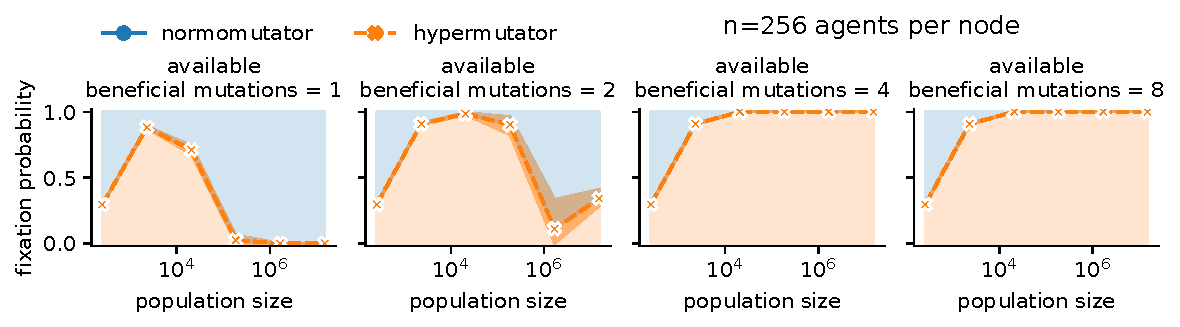
\includegraphics[width=0.8\linewidth]{binder/binder-wse-5050-spatial2d-2048atile-traits.ipynb/binder/teeplots/wse-5050-spatial2d-2048atile-traits/col=available-beneficial-mutations+errorbar=ci+hue=genotype+style=genotype+viz=size-fixation-areaplot+x=population-size+y=fixation-probability+ext=.pdf}%
\vspace{-3ex}
\caption{
\textbf{Restricted adaptive potential favors nonmutators.}
\footnotesize
Area plots show fixation probabilities in WSE simulations initialized with even mix of mutator and nonmutator genotypes.
As available beneficial mutations increase, mutattors gain favor in progressively larger populations.
% Simulations were conducted on WSE using the counter-based genome model, with populations initialized to a 50/50 mix of non- and mutators.
% Subpopulations comprised 2,048 agents per PE.
Shaded bands show bootstrapped 95\% confidence intervals.
% Supplementary Figure \ref{fig:fixheat-wse-altatile:2048} details results in a tabular format.
}
\label{fig:avail-ben-muts}

\vspace{-3ex}

\end{figure}


\section{Introduction} \label{sec:introduction}

% Mutation rates in microbial populations reflect a fundamental evolutionary trade-off.
While mutations are typically orders of magnitude more likely to harm than to help fitness,
%, so low mutation rates increase the proportion of offspring that are viable.
in rare instances, mutation can introduce new beneficial traits.
% \citep{zeyl2004capturing,rozen2002fitness}.
Within asexual populations, such beneficial mutations can set into motion a winner-takes-all scenario where lineages unable to achieve comparable fitness gains are eventually driven to extinction.
% Hence, mutation can confer a rare --- but profound --- fitness benefit.

Like other phenotypic characteristics, the mutation rate of an organism can be strongly influenced by heritable traits --- for instance, by genes for DNA mismatch repair. %\citep{miller1998mutators}.
% Absent ongoing adaptive evolution, purifying selection will tend to suppress so-called ``mutator'' alleles.
In asexual populations lacking recombination, mutator alleles can  ``hitch-hike'' when a fitness-advantaged strain sweeps to fixation and carries along its full genetic background.
% In fact, as mutator alleles can systematically accelerate the pace of adaptive evolution \citep{orr2000rate}, they can even become evolutionarily favored due to generating linked beneficial alleles.
Understanding how and why mutator traits fix has broad importance in our understanding and management of evolving populations.
% Mutator traits have been shown to broadly influence the balance between selection and random effects on genetic content, profoundly accelerating processes of genetic drift \citep{couce2017mutator}.
% In particular, mutator strains can facilitate acquisition of novel pathogen traits such as antibiotic resistance, tumor progression, and changes in virulence.
% \citep{eliopoulos2003hypermutation,jolivetgougeon2011bacterial,stern2016viral,schlesner2015hypermutation,hammerstrom2015acinetobacter,perron2010hypermutability}.
For instance, the emergence of mutator strains has been associated with treatment using antibiotics of last resort \citep{mehta2019essential}.
% Spatial structure associated with biofilms, in particular, has been implicated in facilitating the evolution of antibiotic resistance \citep{france2018spatial}.
% Thus, beyond theoretical interest, studying mutator dynamics has concrete practical applications with real-world potential to benefit both individual health and public well-being.

Existing modeling work has established that large population size, in particular, can drive the probability of mutator traits fixing to near certainty \citep{raynes2018sign,tenaillon1999mutators}.
However, questions remain as to conditions that stabilize very large asexual populations \textit{against} mutator fixation \citep{raynes2019migration}.
Among other findings, reported work has allowed exploration of the role of mutational supply in curtailing mutator advantage at large population sizes (Figure \ref{fig:avail-ben-muts}), as well as the sensitivity of this effect to population structure and background rates of mutator allele prevalence.

% \subsection{Causes and Consequences of Mutator Strains}

% Mutator strains are observed across a wide variety of populations, including both natural systems and laboratory experiments \citep{sniegowski1997evolution,swings2017adaptive,maddamsetti2020divergent,cherry2018methylation,notleymcrobb2002enrichment,shaver2002fitness,voordeckers2015adaptation,leclerc1996high}.
% As such, a substantial body of literature has investigated the conditions under which mutator traits tend to arise.
% As mentioned above, population size has been implicated as a key factor for mutator fixation, as large populations provide more opportunities for the beneficial mutations that drive mutator hitch-hiking \citep{chao1983competition}.
% On the other hand, bottleneck events that suddenly reduce population size can suppress mutator fixation by disrupting propagation of the beneficial alleles that mutators hitchhike off of \citep{raynes2013effect}.

% A wide variety of computational and mathematical modeling approaches have been applied in studying the evolutionary dynamics of mutator alleles.
% Although tangential to the present work, mathematical and computational investigations have notably treated a broad variety of additional topics, including coevolutionary pressures \citep{pal2007coevolution} and interactions with sexual recombination \citep{johnson1999beneficial}.
% Within the purifying selection regime (i.e., absent positive selection for beneficial traits), modeling work has also investigated the interplay between mutator alleles and Muller's ratchet \citep{soderberg2011kickstarting} and dynamics steering towards evolutionarily stable mutation rates \citep{lynch2008cellular}.

% Of more direct salience to present work, \citet{desai2011balance} provide a key foundation in understanding transient fluctuations in mutator allele prevalence, who focus on a dynamic (rather than steady-state) framing of the topic.
% For scenarios with positive selection, attention is first paid to the probability for a given \textit{de novo} beneficial mutation to survive drift effects and reach sufficient frequency to be reliably selected upon.
% Principled approximations are applied to suggest parameter regimes where establishment probability for beneficial alleles arising on a mutator background may safely be considered to be essentially zero (i.e., mutator incurs catastrophic mutational load) and where establishment probability is essentially indistinguishable from nonmutators (i.e., mutator incurs negligible mutational load).
% At these extrema, mutator fixation probability is shown to follow easily from establishment probabilities under the condition that fixation time may be assumed sufficiently short to neglect the possibility of competition between more than one established allele.
% However, in scenarios where either (1) fixation times are long (e.g., large population size) or (2) the mutational load incurred by mutators falls within an intermediate parameter range, matters are noted to become substantially more involved.
% At this point, \citet{desai2011balance} conclude their analysis with a heuristic discussion outlining expected qualitative regimes within these remaining regions of parameter space.
% In line with themes explored in present work, \citet{desai2011balance} note that where fixation times for mutator alleles hitch-hiking with a given beneficial mutation are sufficiently long, establishment of a commensurate beneficial mutation among nonmutators prior to fixation becomes inevitable.
% Therefore, successive adaptive mutations become necessary in such cases to fix a mutator allele.

% Several earlier works provide further insight into the role of adaptive potential in the evolutionary dynamics of mutator alleles.
% The core dynamic by which successive adaptive mutations can ultimately fix a mutator allele is demonstrated by \citet{tanaka2003evolution}.
% Through a combination of analytical and computational modeling, they show how mutator alleles can rise in frequency over the course of a selective sweep for a single beneficial mutation, even if nonmutators are first to discover the beneficial mutation.
% Although beyond the scope of their analyses, it is noted that such an effect could compound over successive adaptive sweeps to boost mutator prevalence.
% Somewhat relatedly, \citet{travis2002mutator} apply a deterministic model to show that mutator concentration can creep progressively above baseline equilibrium when adaptive potential associated with environmental changes becomes available.
% Most pertinently, however, \citet{tenaillon1999mutators} directly demonstrate mutator ratcheting over successive sweeps in a set of extensive finite-sized stochastic simulations, which apply efficient compartment-based representations to model the genetic composition of large well-mixed populations.
% In their simulations, time series traces of mutator proliferation from background levels exhibit clear multistep dynamics.
% Of particular note, simulations using a fixed population size of $10^9$ demonstrate the fixation probability of mutators to increase with the number of adaptive mutations available.

% Recent \textit{in vivo} experimental work has established direct evidence for connections between adaptive potential and mutator outcomes.
% In this work, \citet{callens2023hypermutator} conducted treatments exposing populations of \textit{E. coli} to either antibiotic or osmotic stressors, calibrated to comparable severities.
% Because the antibiotic agent employed in experiments targeted a pathway involving relatively few genes, fewer loci exhibited adaptive potential compared to the large number of pathways implicated by the osmotic stress condition.
% In line with theoretical expectations, the high-adaptive-potential osmotic stressor induced significantly higher rates of mutator fixation.
% More broadly, existing work has drawn clear connections between elevated mutation rate and long-term environmental, coevolutionary, or ecological fluctuations that introduce a moving evolutionary target \citep{leigh1970natural,travis2002mutator,travis2004mutators,rosenbloom2014frequencydependent,pal2007coevolution,wei2022rapid}.

% In a separate vein of inquiry, work by \citet{raynes2018sign} is notable in establishing a systematic understanding of the impact of population size on mutator allele favorability.
% Through paired agent-based simulation and yeast-model experiments, a striking sign-change effect is demonstrated to play out along the spectrum of population size.
% A quantitative basis for this effect is provided by synthesizing independent analytical approximations for the probability of mutator fixation by drift and hitchhiking.
% For small population sizes, mutator alleles' selective cost of imposed deleterious load outweighs their selective benefit in facilitating the discovery of beneficial mutations.
% In larger population sizes, the relative magnitude of these effects switches and mutator alleles become favored via indirect selection for generated beneficial mutations.

% Earlier work has also pointed to the role of population size influencing selection on mutators.
% \citet{wylie2009fixation} apply stochastic simulation and diffusion-based analytical methods to study mutator dynamics in asexual populations, partly describing how large population size can favor mutators.
% A similar conclusion is reached by \citet{andre2006evolution}, through analytical models based in game theory.
% Work by \citet{good2016evolution}, notable for extending analytical modeling efforts into the parameter regime where clonal interference between competing beneficial mutations is at play, also predicts population size to increase fixation probability within well-mixed populations.
% This prediction is validated through forward-time Wright-Fisher simulations.
% (Other aspects of this work are notable in considering effects of mutator alleles on population-level adaptation rates and transient overshooting of evolutionarily stable mutation rates.)

% In this work, we seek to extend understanding of how limited adaptive potential interacts with population size and structure to influence mutator dynamics within asexual populations.
% As noted earlier, such knowledge is needed to improve explanation of how nonmutator alleles can be maintained within large populations.
% In \citep{raynes2018sign}, concluding remarks hypothesize that spatial structure may help to explain why mutator alleles do not universally fix within large asexual populations.
% However, in a later set of paired \textit{in vivo}/\textit{in vitro} experiments, deviation from well-mixed conditions is contradictorally linked to \textit{higher} probability for mutator fixation if any level connectivity remains between subpopulations \citep{raynes2019migration}.
% A simple explanation is provided for this result: although mutators are disfavored within the small population size of an isolated deme, a fixed mutator within any single deme will subsequently invade all remaining demes due to outcompeting nonmutator strains in accruing subsequent adaptive potential.
% Thus, long-term nonmutator persistence requires short-term mutator extinction within \textit{all} subpopulations, such mutator extinction becomes increasingly unlikely with high deme counts.
% In this work, we hypothesize that an opposite effect will occur where adaptive potential is limited.
% Under such a scenario, long-term nonmutator persistence requires short-term nonmutator survival within only a single subpopulation, which can successfully invade mutator subpopulations due to lower mutational load once available adaptive potential is exhausted.

% \subsection{Major Results}

% In our initial experiment, we confirmed that large populations favor mutator fixation, under the assumption of unlimited adaptive potential.
% Consistent with expectations, we found that restricting adaptive potential by capping available adaptive mutations reversed outcomes in large populations to favor nonmutators.
% Investigating the influence of population structure and composition, we found spatial structure to substantially increase the amount of adaptive potential required to fix mutator alleles in large populations.
% However, this effect only occurred when mutator alleles were initially rare within the population.
% We also report qualitative differences between effects of population size on mutator fixation probability under well-mixed versus 2D population structure when mutations are rare.
% In the final part of our investigation, we analyze the spatiotemporal dynamics of our simulations to better understand the mechanisms at play behind these effects.

% Differing from existing results, we find that in the situation of limited adaptive potential, the effect of population structure on fixation probability is actually opposite to that predicted under the theory.
% Population structure has also been found to influence mutator outcomes, with deviation from well-mixed conditions being linked to a higher probability for hypermutator fixation so long as any connectivity remains between subpopulations \citep{raynes2019migration}.

% Of technical note, the large-scale simulations necessary for this work were made possible by exploiting hardware accelerator platforms --- specialized high-performance computing (HPC) peripherals capable of massive computational workloads.
% In line with existing work applying Graphics Processing Units (GPUs) for agent-based modeling \citep{turpin2021xaevol,kosiachenko2019mass,perumalla2009switching,heinemann2007artificial,richmond2023flame}, we found a substantial performance boost: in our case, $378\times$ speedup over single-core CPU evaluation.
% \footnote{%
% Other notable approaches to large-scale evolution simulations have used more traditional cluster-based CPU modeling \citep{moreno2022best,collier2015large,ray1995proposal,turpin2020paevol}, sampling-based approximations \citep{taddei1997role}, and compartmental representations \citep{tenaillon1999mutators}.}
% We also leveraged Wafer-Scale Engine (WSE) technology in this work, a cutting-edge AI/ML-oriented platform that delivers 850,000 processor cores packed together on a single chip.
% Simulation on WSE achieved a further $294\times$ speedup, resulting in a net $111{,}091\times$ speedup from single-CPU evaluation.
% These performance gains ultimately benefited the work by allowing us to employ forward-time agent-based simulation at full resolution across genome models and population structures that are difficult to integrate with compartment-based approaches used for simulations of large populations in existing work.

% These performance gains ultimately benefited the work by allowing us to employ forward-time agent-based simulation at full resolution across genome models and population structures that are difficult to integrate with compartment-based approaches used for simulations of large populations in existing work.

To enable the simulation scale necessary for this work, we employed Graphics Processing Unit (GPU) and Wafer-Scale Engine (WSE) hardware accelerators.
The Cerebras CS-2 WSE, in particular, is notable among an emerging class of next-generation AI/ML-oriented hardware accelerators.% \citep{lauterbach2021path}.
This chip comprises a grid lattice of 850,000 independent processor elements (PEs), networked for low-latency communication among neighboring PEs.
Explorations are ongoing in establishing applications of these platforms for scientific and high-performance computing (see e.g., \citep{rocki2020fast,ltaief2023scaling,sai2023massively}).

Notably, however, major challenges exist in adapting simulation codes to the WSE platform's dataflow paradigm and extreme constraints in memory use and communication locality.
At the hardware level, all communication occurs through message passing between directly adjacent processing tiles.
Additionally, although on-device memory totals nearly 50GB, only 48kb is available per PE.
We address these constraints by mapping WSE layout to simulation spatial structure and adopting dynamic data coarsening strategies, discussed next.
In concert with traditional observational and experimental work, harnessing such next-generation hardware accelerator platforms promises to ultimately contribute in extending biological understanding across broader scales and levels of organization.
%The ability to leverage emerging HPC architectures, as shown here, offers a practical step toward addressing such challenges.


% A key trade-off encountered in this work is in memory constraints imposed by WSE architecture, which supplies only 48kb of memory per PE.

% Of technical note, the large-scale simulations necessary for this work were made possible by exploiting hardware accelerator platforms --- specialized high-performance computing (HPC) peripherals capable of massive computational workloads.
% In line with existing work applying Graphics Processing Units (GPUs) for agent-based modeling \citep{turpin2021xaevol,kosiachenko2019mass,perumalla2009switching,heinemann2007artificial,richmond2023flame}, we found a substantial performance boost: in our case, $378\times$ speedup over single-core CPU evaluation.
% \footnote{%
% Other notable approaches to large-scale evolution simulations have used more traditional cluster-based CPU modeling \citep{moreno2022best,collier2015large,ray1995proposal,turpin2020paevol}, sampling-based approximations \citep{taddei1997role}, and compartmental representations \citep{tenaillon1999mutators}.}
% We also leveraged Wafer-Scale Engine (WSE) technology in this work, a cutting-edge AI/ML-oriented platform that delivers 850,000 processor cores packed together on a single chip.
% Simulation on WSE achieved a further $294\times$ speedup, resulting in a net $111{,}091\times$ speedup from single-CPU evaluation.



% In the CORE of our experimental work, we sought to establish how adaptive potential interacts with current synthesis of the role of population size in mediating mutator dynamics.
% This involved conducting a series of trials across WSE,
% Due to the inherent spatial structure owing to local connectivity on the WSE, aspects of experiments were complimented by GPU to provide perspective under well-mixed conditions.

% At the core of these broader experiments is the finding

% Figure \ref{fig:avail-ben-muts} shows fixation curves where one, two, three, four, and five beneficial mutations are available, conducted with 256 agents per deme.
% Under surveyed conditions, with 2D spatial structure and mutators initially in equal proportion to nonmutators, nonmutator persistence rapidly decays with increases in adaptive potential.
% Even with the largest surveyed billion-agent population size, mutators regain selective parity where four or more beneficial mutations are available.

% One assumption of existing work by \citet{raynes2018sign} is availability of abundant potential beneficial mutations.
% Existing simulation studies suggest that restricting adaptive potential should disfavor mutator alleles \citep{tenaillon1999mutators}, but understanding of how this effect interacts with other factors is limited.

% To investigate this question, we performed experiments where the supply of possible beneficial mutations was constrained.
% Experiments were conducted on the WSE platform using 2D population structure with 50/50 initialization.
% The right panels of \cref{fig:wse-inf-one:32,fig:wse-inf-one:2048} show mutator fixation probabilities where agents could accrue no more than one beneficial mutation for trials using 32 and 2,048 agents per deme, respectively.
% In both cases, a second sign-change fitness effect for mutator traits appears, with nonmutators regaining favor past population sizes of 100,000 agents.
% Beyond population sizes of 1 million agents, nonmutators reliably drive mutators to extinction.

% These results substantiate an earlier verbal hypothesis by \citet{desai2011balance} that more than one beneficial mutation should become necessary to fix a mutator allele when fixation time becomes long, as is the case with large population size.
% The rationale behind this expectation is that where fixation time is long, non-mutators are more likely to discover a comparable beneficial allele before being driven to extinction.
% From this point, disadvantage in mutational load dooms the mutator allele.




% Next, we tested sensitivity of the relationship between mutator fixation probability and population size with respect to the amount of adaptive potential available.

% Interestingly, this result may help explain an earlier observation by \citet{tenaillon1999mutators} that below a threshold of four beneficial mutations available, mutator alleles never rose from background levels to fix within their compartment-based model of a well-mixed billion-member population.
% Notwithstanding differences in model parameterization and population structure, our findings suggest that this threshold may coincide with the point where the net fitness effect of the mutator allele neutralizes in commensurately scaled populations.


\section{Simulation Model and Implementation} \label{sec:methods}

% Experiments were conducted \textit{in silico} using stochastic agent-based modeling approaches.
Our simulations tracked fixed-capacity populations of discrete agents propagated in synchronous generations, with competition between agents to create asexual offspring.
Each agent possessed a set of genetic traits, inherited subject to mutation, that influenced reproductive success; mutator strains were subjected to 100$\times$ higher mutation rates.
Our genome model tracked counts of accumulated beneficial and deleterious mutations, following closely from \citep{raynes2018sign}.
To assess the generality of our findings, we supplemented this simple ``counter-based'' genome model with an alternate ``site-explicit'' genome model where beneficial mutations become rarer as adaptation unfolds.
% These genome models are described below.
%
% This section reviews the model mechanics used across experiments in this work, as well as aspects of simulation design used to enact treatment conditions.
% Experimental variables varied between treatments include population size, spatial population structure, background prevalence of mutator traits, and restriction of adaptive potential.
% Finally, we describe notable implementation-level considerations necessary in harnessing high-performance computing hardware to achieve the simulation of large, heterogeneous populations necessary for this work.
%
% \subsection{Counter-based Genome Model} \label{sec:poisson}
%
% Primary experiments in this work apply an agent-based modeling approach closely following work by \citet{raynes2018sign}.
% We also adopt parameters from \citet{raynes2018sign}, which were chosen on the basis of values reported from laboratory measurements on \textit{E. coli} strains\citep{wloch2001direct,frenkel2014fates,joseph2004spontaneous,levy2015quantitative,zeyl2001estimates}.
% Under the ``counter-based'' framework, agent genomes consist of two counters: one tracking beneficial mutations accumulated ($n_b$) and the other tracking deleterious mutations accumulated $n_d$.
% As modeled in several pieces of related work \citep{tenaillon1999mutators,travis2002mutator,raynes2019migration,tanaka2003evolution,wylie2009fixation}, mutations are assumed to have comparable fitness impacts.
% Thus, a genome's ``fitness score'' is calculated simply as $n_b - n_d$.
% (Details on how ``fitness score'' influences selection are described in Section \ref{sec:evolution}.)
% For purposes here, the simplicity of this approach is useful in enabling runtime simulation efficiency.
% Sensitivity analysis performed in closely related work applying this genome model found evolutionary outcomes to be similar to those with exponential distributions of fitness effects for individual mutations \citep{raynes2019selection}.
%
% Genomes were subjected to mutation each generation.
% For each offspring, counts of newly accrued beneficial and deleterious mutations are drawn from independent Poisson distributions.
% Expected deleterious mutations per generation were parameterized as
% $\lambda_d=10^{-3}$ and expected beneficial mutations per generation were parameterized as $\lambda_b=10^{-6}$.
% Reversions are not considered, so beneficial and deleterious mutation counts are strictly nondecreasing.
% In some experiments where adaptive potential was limited, we imposed an upper bound on the maximum quantity of beneficial mutations available.
% Any further beneficial mutations accrued past this point were reverted to the bound.
%
% Agent genomes additionally contain a boolean flag, signifying whether the agent expresses a mutator trait.
% Agents with this trait incur a hundred-fold increase to mutation rates, $\hat{\lambda_d} = 100 \times \lambda_d$ and $\hat{\lambda_b} = 100 \times \lambda_b$.
% We assume no direct fitness benefit or cost to be associated with the mutator allele.
%
% Experiments applied one of two approaches to introduce mutator alleles.
% In the ``50/50'' treatment, genomes were initialized equiprobably as a mutator or as a nonmutator.
% The ``50/50'' experiment design, applied in \textit{in vivo} experiments reported in \citet{raynes2018sign}, maximizes sensitivity in detecting sign-change fitness effects where selection transitions between favoring versus disfavoring mutator alleles.
% Rationale behind this approach also stems from the understanding that fitness effects from mutator alleles act in a density- and count-independent manner \citep{raynes2019selection}.
% By contrast, in other experiments, we introduced mutator alleles via a \textit{de novo} approach where the mutator trait is spontaneously conferred to offspring with probability $10^{-6}$.
% Under this approach, the founding population is initialized as nonmutator type.
% As with prior work \citep{raynes2018sign}, neither treatment allows mutator to nonmutator reversion.
%
% \subsection{Site-explicit Genome Model} \label{sec:site-explicit}
% As originally formulated in \citet{raynes2018sign}, the counter-based genome model assumes the availability of an unlimited adaptive potential.
% In particular, the memorylessness of the probability distribution for mutation accumulation suits the assumption that an unlimited number of beneficial (or deleterious) mutations are available.
% To better reflect scenarios with limited adaptive potential, we replicated several experiments using a genome model explicitly designating a finite set of loci with adaptive potential.
% The major consequence of such a ``site-explicit'' model is that discoverable beneficial mutations become scarcer, and hence more difficult to discover, as adaptation unfolds.

% Under the site-explicit approach, we model genomes as containing a discrete, finite set of $n$ loci $b_i \in \{0, 1\}$ available for adaptive mutation.
% All loci are initialized $b_i = 0$.
% When inherited, loci transition $0 \rightarrow 1$ with probability $p_b = 10^{-6}$, representing acquisition of a beneficial mutation.
% Reversion mutations $1 \rightarrow 0$ are allowed, also with probability $p_{\sim b} = 10^{-6}$.

% Because we do not limit the quantity of available deleterious mutations in our simulations, we maintained a counter-based approach in tracking deleterious mutations, with deleterious mutation acquisition Poisson distributed $\lambda_d = 10^{-3}$.
% Hence, under the site-explicit model, we assign agents' fitness scores as $-n_d + \sum^n b_i$.

% Mutator allele mechanics under the site-explicit model closely follow the counter-based model.
% The mutator trait increases mutation rates hundredfold, setting $\hat{p_{b}} = \hat{p_{\sim b}} = 10^{-4}$ and $\hat{\lambda_d} = 10^{-1}$.
% Site-explicit experiments were conducted under both ``50/50'' and ``\textit{de novo}'' models of mutator introduction, identically to description above.

% \subsection{Evolution Model} \label{sec:evolution}

% Simulations applied a tournament selection strategy with synchronous generations and fixed population size.
% For each available slot in a subpopulation's next generation, we sampled, with replacement, a pair of candidate parents from that subpopulation.
% With 90\% probability, a selected parent is chosen randomly among the pair.
% Otherwise, the candidate with the higher fitness score was selected as the parent.
% As such, fitness score improvements conferred a 10\% fitness advantage.
% Our motivation in performing selection via pairwise competition was to enable efficient vectorized operations for GPU evaluation.

% In simulations with spatial structure, populations were partitioned into well-mixed 256-agent ``demes.''%
% \footnote{%
% Where noted, 32-agent and 2,048-agent deme sizes were also used, to support finer-grained sweeps of population size or higher maximum net population size.
% }
% Where deme structure was used, competition occurred only between agents inhabiting the same deme.
% Each generation, migration between neighboring demes was applied by swapping a pair of agents.
% Hence, demes received one immigrant from each neighbor per generation.
% Under default conditions, demes were arranged as a two-dimensional grid lattice with non-toroidal boundaries (i.e., grid edges did not wrap around).
% For well-mixed treatments, deme structure was broken down to treat entire populations as a single deme.

% Our 2D structure experiments used square deme grids.
% To maintain square layout, we scaled surveyed population sizes by factors of 9: $1 \times 1 \times 256,\;\; 3 \times 3 \times 256,\;\; 9 \times 9 \times 256,\;\; \ldots,\;\; 729 \times 729 \times 256$.
% To efficiently batch our computations, we processed smaller population sizes as independent tiles of a larger, fixed-size fabric.
% Hence, replicate count decreased with population size, but was boosted to at least 9 replicates in all cases.
% Simulations lasted 500,000 generations, which sufficed for populations to reach fixation in nearly all cases.
% (We defined fixation as all mutators or all nonmutators for 50/50 experiments, and as either 100\% mutators or <1\% mutators for \textit{de novo} experiments.)
% However, we found that 256-agent populations failed to reliably reach full adaptive potential in accruing more than 12 beneficial mutations within the prescribed 500,000 generation window.
% Thus, we excluded 256-agent simulations with more than 12 beneficial mutations available from our analyses.

% For all included data, $>97\%$ of replicates reached both mutator/nonmutator fixation and accrued full adaptive potential.
% Details on the fraction of replicates reaching fixation by experimental condition are provided in Supplementary \cref{fig:neither-fixed-5050-cupy,fig:neither-fixed-denovo-cupy,fig:neither-fixed-wse-256atile,fig:neither-fixed-wse-altatile}.
% Details on the fraction of replicates reaching full adaptive potential, measured for GPU-based simulations, appear in Supplementary \cref{fig:unaccrued-5050-cupy,fig:unaccrued-denovo-cupy}.

% \subsection{Hardware Accelerator Platforms} \label{sec:hardware}

% \subsection{Kernel Design} \label{sec:kernel}

To suit the local lattice structure of the WSE's hardware architecture, all experiments on this platform employed 2D spatial population structure.
Each PE hosted a single subpopulation, acting as an ``island.''
Thus, in trials configured with 2,048 agents per PE, net population size reached 1.5 billion agents.
Agents migrated between neighboring PEs via asynchronous message passing;
% see e.g.,
% https://github.com/mmore500/wse-async-ga/blob/ebc92bd012f0bb31092c5e71825af041261c35c5/kernel-async-ga/kernel.csl
% and
% https://osf.io/esv9z
% (note that send flag is bumped twice per send cycle)https://osf.io/esv9z
in practice, each PE dispatched approximately one agent to each neighbor per generation.
Progress of each PE in stepping through agent generations within its own subpopulation was allowed to proceed independently of other PEs.
Other detail on the Cerebras Software Language (CSL) kernel design adapted for this work is provided in \citet{moreno2024trackable}.

% In some cases, experiments on WSE were extended beyond the $729 \times 729$ deme configuration to fill the CS-2 WSE's entire $750 \times 994$ complement of available PEs.

% For a set of supplementary trials described in Section \ref{sec:dynamics}, we applied additional runtime data logging in our simulations to track time series data of mutator allele prevalence.
% Generation-on-generation, we configured each processor element to sample a genome from its local population and record its mutator allele status (i.e., a binary value as either a non- or mutator).
% To efficiently curate this single-bit data within per-PE memory limits while allowing a flexible recording duration, we leveraged recently introduced ``DStream'' ring buffer data structures \citep{moreno2024algorithms}.
% Notably, this approach constrained memory use to a fixed-size buffer, while allowing recording to be dynamically halted when nonmutators were determined to be locally extinct (and restarted if they are reintroduced).
% While this scheme allowed maximization of on-device resources, as a consequence the set of sampled time points varied depending on how long nonmutator alleles persisted.
% As a result, the number of generations elapsed per frame in provided animations varies. Availability


% Given the stochastic nature of agent-based evolution models, our experiments relied heavily on pseudorandom number generators (PRNGs).
% These algorithms emulate true entropy by producing a sequence of output values that, although deterministic, are statistically independent.
% Due to performance engineering considerations, vendor-supplied PRNG implementations for the WSE and GPU do not employ cryptographic-quality algorithms.
% Our WSE simulations relied on Cerebras Software Language's PRNG utilities, which use a Linear-Feedback Shift Register (LFSR) approach with polynomial $3x^2 + 8x + 1$ strided by 128 iterations.
% On GPU, we used CuPy's PRNG utilities, which expose CUDA's underlying XORWOW-based CuRAND implementation \citep{marsaglia2003xorshift}, another type of LFSR approach \citep{brent2004note}.

% PRNG patterning, particularly in lower-quality Linear Congruential Generator (LCG) algorithms, has been shown in some cases to substantially bias simulation results \citep{click2010quality}.
% Notably, we encountered one set of conditions in WSE simulations where fixation probabilities for 12 beneficial mutations available deviated appreciably from that for 10 and 14 beneficial mutations.
% The anomaly occurred solely under the site-explicit genome model, where the number of PRNG calls made to apply mutation to an agent differs with the quantity of available beneficial mutations.
% In the anomalous configuration, each PE comprised a fully independent population, so replicate count was very high ($n = 827 \times 827 = 683,929$), making the result all the more unexpected.

% Fully re-running the affected simulation did not resolve the data anomaly.
% However, modifying the simulation code to advance the PRNG engine via no-op calls within the body of the mutation operator brought the result in line with expectations.
% Thus, it seems likely that, in this instance, the simulation encountered a PRNG cycle or similar artifact.
% As such, for this data point, we exclude the originally generated data in favor of the results with added PRNG stepping.
% We note that on a more general basis, the soundness of our simulation implementations is bolstered by consistency between similar experiments conducted on WSE and GPU.
% In particular, CuRAND's RNG has been extensively characterized and, although it exhibits statistically detectable flaws of its own, is considered to be of production quality \citep{nvidia2024curand}.
% Given the stochastic nature of agent-based evolution models, our experiments relied heavily on pseudorandom number generators (PRNGs).
% These algorithms emulate true entropy by producing a sequence of output values that, although deterministic, are statistically independent.
% Due to performance engineering considerations, vendor-supplied PRNG implementations for the WSE and GPU do not employ cryptographic-quality algorithms.
% Our WSE simulations relied on Cerebras Software Language's PRNG utilities, which use a Linear-Feedback Shift Register (LFSR) approach with polynomial $3x^2 + 8x + 1$ strided by 128 iterations.
% On GPU, we used CuPy's PRNG utilities, which expose CUDA's underlying XORWOW-based CuRAND implementation \citep{marsaglia2003xorshift}, another type of LFSR approach \citep{brent2004note}.

% PRNG patterning, particularly in lower-quality Linear Congruential Generator (LCG) algorithms, has been shown in some cases to substantially bias simulation results \citep{click2010quality}.
% Notably, we encountered one set of conditions in WSE simulations where fixation probabilities for 12 beneficial mutations available deviated appreciably from that for 10 and 14 beneficial mutations.
% The anomaly occurred solely under the site-explicit genome model, where the number of PRNG calls made to apply mutation to an agent differs with the quantity of available beneficial mutations.
% In the anomalous configuration, each PE comprised a fully independent population, so replicate count was very high ($n = 827 \times 827 = 683,929$), making the result all the more unexpected.

% Fully re-running the affected simulation did not resolve the data anomaly.
% However, modifying the simulation code to advance the PRNG engine via no-op calls within the body of the mutation operator brought the result in line with expectations.
% Thus, it seems likely that, in this instance, the simulation encountered a PRNG cycle or similar artifact.
% As such, for this data point, we exclude the originally generated data in favor of the results with added PRNG stepping.
% We note that on a more general basis, the soundness of our simulation implementations is bolstered by consistency between similar experiments conducted on WSE and GPU.
% In particular, CuRAND's RNG has been extensively characterized and, although it exhibits statistically detectable flaws of its own, is considered to be of production quality \citep{nvidia2024curand}.
% \subsection{On-hardware Simulation Performance}
% \label{sec:performance}

% \begin{figure}

% \begin{subfigure}{0.5\textwidth}
% 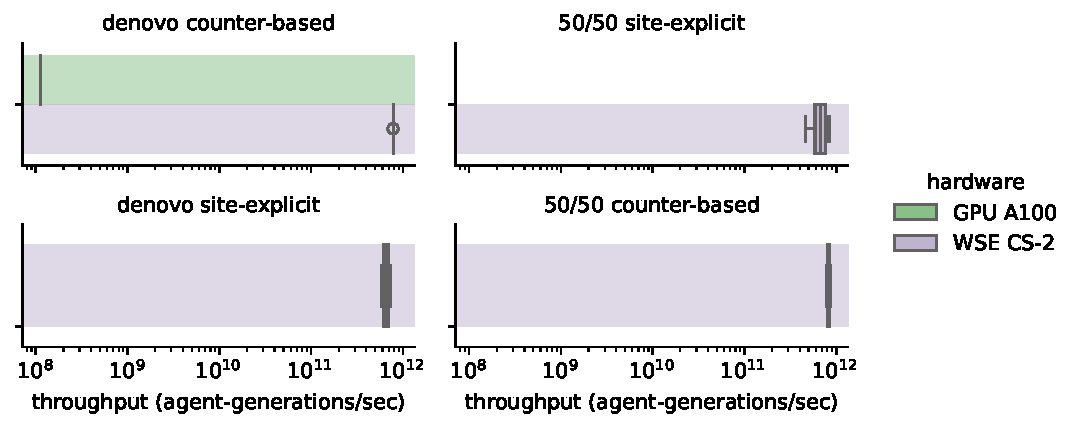
\includegraphics[width=\textwidth, trim={0cm 0cm 2.5cm 0cm}, clip]{binder/binder-perf-wse-vs-gpu.ipynb/binder/teeplots/col=experiment-design+hue=hardware+orient=h+viz=backplot+x=throughput-agent-generations-sec+ext=.pdf}
% \caption{throughput}
% \label{fig:perf:throughput}
% \end{subfigure}%
% \begin{subfigure}{0.49\textwidth}
\centering
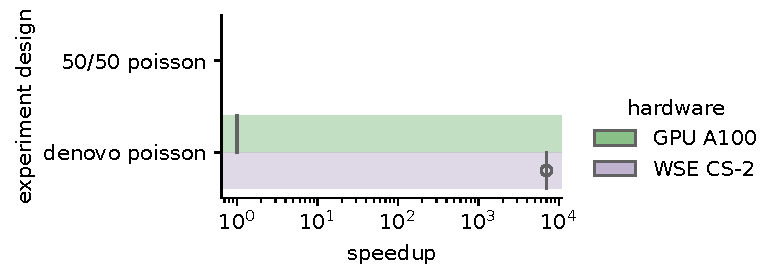
\includegraphics[width=0.85\linewidth]{binder/binder-perf-wse-vs-gpu.ipynb/binder/teeplots/hue=hardware+orient=h+viz=backplot+x=speedup+y=experiment-design+ext=.pdf}

\vspace{-2ex}
% ~
% \caption{speedup}
% \label{fig:perf:speedup}
% \end{subfigure}

\caption{
  \textbf{CPU, GPU, and WSE simulation performance.}
  \footnotesize
  CPU throughput was measured from NumPy-backed simulation code, GPU throughput was measured from equivalent CuPy-backed simulation code, and WSE throughput was measured from a comparable Cerebras Software Language implementation.
  CPU experiments were single-core on AMD EPYC 7H12 (2.595 GHz), GPU hardware was NVIDIA A100 hosted by AMD EPYC 7713 (2.0 GHz) or Intel Xeon 8358 (2.6 GHz), and WSE hardware was CS-2 hosted by Intel Xeon Platinum 8280L (2.7-4.0 GHz).
  Speedup was calculated relative to mean CPU throughput.
  % Shaded areas indicate bootstrapped 95\% confidence intervals with sample size $\geq 10$.
}
\label{fig:perf}
\end{figure}


% To assess the efficacy of hardware accelerator resources in expediting our simulations, we collected timings of runtime duration from our simulation experiments.
% As a baseline comparison point for performance, we also benchmarked simulation on CPU (AMD EPYC 7H12 2.595 GHz).

% Figure \ref{fig:perf} compares simulation performance between hardware platforms, measured in agent-generations per second (AGPS).
% Mean throughput was 7.0 (SD 0.5) million AGPS on CPU, 2.7 (SD 0.03) billion AGPS on GPU, and 780 (SD 0.5) billion AGPS on WSE for \textit{de novo} trials using the counter-based model.
% Net speedup, normalized to mean CPU throughput, was $378\times$ (SD 4) on GPU and $111,091\times$ (SD 75) on WSE.
% Normalized to net GPU performance, WSE provided a speedup of $294\times$ (SD 0.2).

% Under the site-explicit model, WSE gave 650 (SD 50) billion AGPS under \textit{de novo} conditions.
% The site-explicit model was not implemented on GPU.
% For all the above, 50/50 trials gave similar performance to \textit{de novo}.

% On WSE, we found agent-generation throughput to be generally consistent across per-PE population densities, as shown in Supplementary Figure \ref{fig:perf-tilepop}.
% In contrast, mean GPU throughput dropped $>95\%$ to 121 million AGPS when increasing net population size from 15.1 million to 175 million.
% For this reason, we only scaled GPU experiments up to 15.1-million-agent populations ($243 \times 243$ demes).

% \subsection{Software, Data, and Materials} \label{sec:materials}

Simulation code, configuration files, and batch scripts are available via the Open Science Framework at \url{https://doi.org/10.17605/OSF.IO/YMAF8}.
% To enable the simulation scale necessary for this work, we employed Graphics Processing Unit (GPU) and Wafer-Scale Engine (WSE) hardware accelerators, which contain large collections of worker processors specialized for numerical computation.
CPU hardware was AMD EPYC 7H12, GPU hardware was NVIDIA A100, WSE hardware was Cerebras CS-2 \citep{buitrago2021neocortex,Brashear2025}.
%\citep{choquette2021nvidia,cerebras2021wafer}.
% WSE hardware was hosted by the Neocortex at PSC.

% This project benefited significantly from open-source scientific software \citep{2020SciPy-NMeth,harris2020array,reback2020pandas,mckinney-proc-scipy-2010,waskom2021seaborn,hunter2007matplotlib,moreno2023teeplot}.


% \section{Results}
\begin{figure}[ht]
  \centering
  \resizebox{\columnwidth}{!}{%
  \begin{minipage}{\textwidth} %

  %----------------------------
  % First row: NO FIXATION
  \begin{subfigure}[t]{\textwidth}
    \centering
    % Left minipage for row label (empty caption)
    \begin{minipage}[b]{0.04\textwidth}
      \caption{}
      \label{fig:dynamics:no-fixation}
    \end{minipage}
    % Six images (columns)
    \begin{minipage}[b]{0.15\textwidth}
      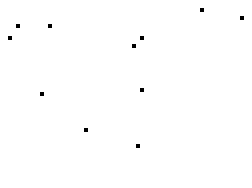
\includegraphics[width=\linewidth]{binder/binder-wse-denovo-spatial2d-explicitsite-timeseries.ipynb/binder/wse-denovo-spatial2d-explicitsite-timeseries/a=traitframes+nmut=14+rep=39a89ca6-a1b5-4b32-ae5f-f0dbb40ba027/dstream_Tbar=000504+ext=.png}
    \end{minipage}
    \begin{minipage}[b]{0.15\textwidth}
      
\includegraphics[width=\linewidth]{binder/binder-wse-denovo-spatial2d-explicitsite-timeseries.ipynb/binder/wse-denovo-spatial2d-explicitsite-timeseries/a=traitframes+nmut=14+rep=5dc8e084-0382-4d7b-9b76-6c3902ca3c1d/dstream_Tbar=000952+ext=.png}
    \end{minipage}
    \begin{minipage}[b]{0.15\textwidth}
      \includegraphics[width=\linewidth]{binder/binder-wse-denovo-spatial2d-explicitsite-timeseries.ipynb/binder/wse-denovo-spatial2d-explicitsite-timeseries/a=traitframes+nmut=14+rep=5dc8e084-0382-4d7b-9b76-6c3902ca3c1d/dstream_Tbar=001400+ext=.png}
    \end{minipage}
    \begin{minipage}[b]{0.15\textwidth}
      
\includegraphics[width=\linewidth]{binder/binder-wse-denovo-spatial2d-explicitsite-timeseries.ipynb/binder/wse-denovo-spatial2d-explicitsite-timeseries/a=traitframes+nmut=14+rep=5dc8e084-0382-4d7b-9b76-6c3902ca3c1d/dstream_Tbar=002552+ext=.png}
    \end{minipage}
    \begin{minipage}[b]{0.15\textwidth}
      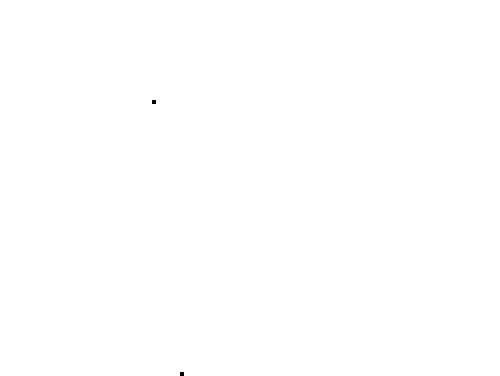
\includegraphics[width=\linewidth]{binder/binder-wse-denovo-spatial2d-explicitsite-timeseries.ipynb/binder/wse-denovo-spatial2d-explicitsite-timeseries/a=traitframes+nmut=14+rep=5dc8e084-0382-4d7b-9b76-6c3902ca3c1d/dstream_Tbar=020472+ext=.png}
    \end{minipage}
    \begin{minipage}[b]{0.15\textwidth}
      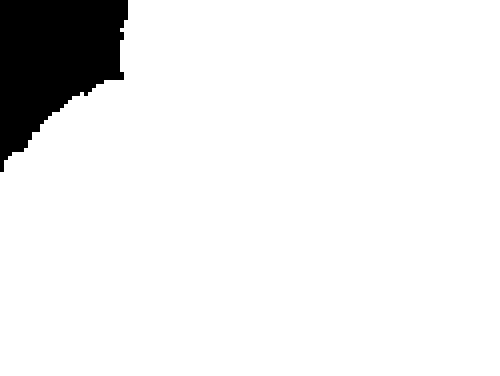
\includegraphics[width=\linewidth]{binder/binder-wse-denovo-spatial2d-explicitsite-timeseries.ipynb/binder/wse-denovo-spatial2d-explicitsite-timeseries/a=traitframes+nmut=14+rep=5dc8e084-0382-4d7b-9b76-6c3902ca3c1d/dstream_Tbar=061424+ext=.png}
    \end{minipage}
  \end{subfigure}

  \vspace{1em} % vertical space between rows

  %----------------------------
  % Second row: FIXATION
  \begin{subfigure}[t]{\textwidth}
    \centering
    % Left minipage for row label (empty caption)
    \begin{minipage}[b]{0.05\textwidth}
      \caption{}
      \label{fig:dynamics:fixation}
    \end{minipage}
    % Six images (columns)
    \begin{minipage}[b]{0.15\textwidth}
      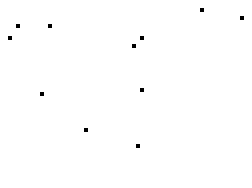
\includegraphics[width=\linewidth]{binder/binder-wse-denovo-spatial2d-explicitsite-timeseries.ipynb/binder/wse-denovo-spatial2d-explicitsite-timeseries/a=traitframes+nmut=14+rep=39a89ca6-a1b5-4b32-ae5f-f0dbb40ba027/dstream_Tbar=000504+ext=.png}
    \end{minipage}
    \begin{minipage}[b]{0.15\textwidth}
      
\includegraphics[width=\linewidth]{binder/binder-wse-denovo-spatial2d-explicitsite-timeseries.ipynb/binder/wse-denovo-spatial2d-explicitsite-timeseries/a=traitframes+nmut=14+rep=39a89ca6-a1b5-4b32-ae5f-f0dbb40ba027/dstream_Tbar=000952+ext=.png}
    \end{minipage}
    \begin{minipage}[b]{0.15\textwidth}
      \includegraphics[width=\linewidth]{binder/binder-wse-denovo-spatial2d-explicitsite-timeseries.ipynb/binder/wse-denovo-spatial2d-explicitsite-timeseries/a=traitframes+nmut=14+rep=39a89ca6-a1b5-4b32-ae5f-f0dbb40ba027/dstream_Tbar=001400+ext=.png}
    \end{minipage}
    \begin{minipage}[b]{0.15\textwidth}
      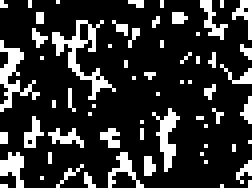
\includegraphics[width=\linewidth]{binder/binder-wse-denovo-spatial2d-explicitsite-timeseries.ipynb/binder/wse-denovo-spatial2d-explicitsite-timeseries/a=traitframes+nmut=14+rep=39a89ca6-a1b5-4b32-ae5f-f0dbb40ba027/dstream_Tbar=002489+ext=.png}
    \end{minipage}
    \begin{minipage}[b]{0.15\textwidth}
      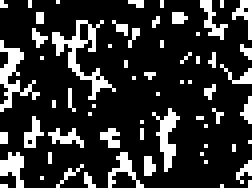
\includegraphics[width=\linewidth]{binder/binder-wse-denovo-spatial2d-explicitsite-timeseries.ipynb/binder/wse-denovo-spatial2d-explicitsite-timeseries/a=traitframes+nmut=14+rep=39a89ca6-a1b5-4b32-ae5f-f0dbb40ba027/dstream_Tbar=002489+ext=.png}
    \end{minipage}
    \begin{minipage}[b]{0.15\textwidth}
      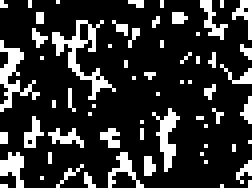
\includegraphics[width=\linewidth]{binder/binder-wse-denovo-spatial2d-explicitsite-timeseries.ipynb/binder/wse-denovo-spatial2d-explicitsite-timeseries/a=traitframes+nmut=14+rep=39a89ca6-a1b5-4b32-ae5f-f0dbb40ba027/dstream_Tbar=002489+ext=.png}
    \end{minipage}
  \end{subfigure}

  %----------------------------
  % Timepoint labels below the bottom row:
  \begin{minipage}[c]{0.154\textwidth}
\hfill
\begin{varwidth}{\textwidth}
$T = 504$
\end{varwidth}
\hfill
  \end{minipage}
  \begin{minipage}[c]{0.154\textwidth}
\hfill
\begin{varwidth}{\textwidth}
$T = 952$
\end{varwidth}
\hfill
  \end{minipage}
  \begin{minipage}[c]{0.154\textwidth}
\hfill
\begin{varwidth}{\textwidth}
$T = 1,400$
\end{varwidth}
\hfill
  \end{minipage}
  \begin{minipage}[c]{0.154\textwidth}
\hfill
\begin{varwidth}{\textwidth}
$T = 2,552$
\end{varwidth}
\hfill
  \end{minipage}
  \begin{minipage}[c]{0.154\textwidth}
\hfill
\begin{varwidth}{\textwidth}
$T = 20,472$
\end{varwidth}
\hfill
  \end{minipage}
  \begin{minipage}[c]{0.154\textwidth}
\hfill
\begin{varwidth}{\textwidth}
$T = 61,424$
\end{varwidth}
\hfill
  \end{minipage}

  \end{minipage}%
  }%

  \caption{
  \textbf{Spatiotemporal composition of simulated populations from Wafer-Scale Engine experiments.}
  \footnotesize
  Snapshots show 191 million agent populations with 2D spatial structure, using site-explicit genome model configured to adaptive potential of 14 beneficial mutations available and mutators introduced \textit{de novo}.
  Raster values are binary, with white pixels indicating a sampled nonmutators and black pixels indicating a sampled mutator.
  Subpanels \ref{fig:dynamics:no-fixation} and       \ref{fig:dynamics:fixation} show replicates where mutators do not, and do, reach fixation, respectively.
  Animations are provided at \url{https://hopth.ru/ej} and \url{https://hopth.ru/ek}.
  Example timecourses for simulations with 12 and 16 beneficial mutations available can be found at \url{https://hopth.ru/el} and \url{https://hopth.ru/em}.
  }
  \label{fig:dynamics}
\end{figure}


\section{On-device Data Management}
\label{sec:dynamics}

% Transient dynamics
% % While this scheme allowed maximization of on-device resources, as a consequence the set of sampled time points varied depending on how long nonmutator alleles persisted.
% % As a result, the number of generations elapsed per frame in provided animations varies.

% To assess how competition between non- and mutator strains unfolds at very large population scales, we performed an additional set of simulations on the WSE using the site-explicit model of adaptation, where mutators originated \textit{de novo} from nonmutator strains.
% For these experiments, a subpopulation size of 256 agents per PE was used to preserve on-device memory to record time series data.
% This configuration yielded a net population size of 191 million agents.
% In these trials, we probed the critical region where outcomes transition between nonmutator and mutator fixation, configuring adaptive potential between 12 and 16 available beneficial mutations.

A key challenge in this work was balancing limited on-device memory between simulation content and data recording.
For example, some experiments required time series measurements of mutator prevalence in PE subpopulations (Figure \ref{fig:dynamics}).
To economize memory use, we applied recently developed algorithms that generalize ring buffer storage to efficiently perform systematic temporal downsampling \citep{moreno2024algorithms,gunther2014algorithm}.
Successive local samples are recorded as single bits within a flat, fixed-size buffer --- with no bookkeeping overhead.
Crucially, because recording duration (i.e., until extinction) is unknown \textit{a priori}, this approach dynamically coarsens recording density via overwrites once storage capacity is reached --- strictly bounding memory use.

% Crucially, given extinction timings are unknown \textit{a priori}, after storage capacity is reached, this approach  a representative online downsample, of configurable composition, is dynamically coarsened once capacity is reached.
% We configured each processor element to sample a genome from its local population and record its mutator allele status (i.e., a binary value as either a non- or mutator).
% However, the duration of recording was not known \textit{a priori}, as it depended on the timing of stochastic fixation events within the simulation itself.
% To efficiently curate this single-bit data within per-PE memory limits while allowing  (as timing of extinction or fixation events is not known \textit{a priori}), we leveraged recently introduced ``DStream'' ring buffer data structures \citep{moreno2024algorithms}.
% Crucially, this approach constrained memory use to a fixed-size buffer known \text{a priori}, while allowing recording to be dynamically halted when nonmutators were determined to be locally extinct (and restarted if they are reintroduced).
% These allowed to be stored in flat memory without data structure overhead, with configurable distribution over time.
Among other results, this data collection strategy revealed that even in circumstances where mutator alleles did not reliably fix, they could nonetheless transiently dominate population composition --- in some cases, reaching peaks upwards of 99.9\% frequency.
% at peak mutator prevalence, nonmutators transiently shrink to less than 0.1\% of population in experiments under conditions where mutators were initially rare but did not fix.
% Given that biological analyses often amenable to incomplete data,

Given limitations in studying real-world systems, biological analyses are often robust to coarsening and sampling.
As such, we see significant opportunity in future work to more broadly explore how such best-effort data collection approaches can be applied to meet practical constraints of hardware accelerator device architectures.
%  which we are interested in continuing to explore in future work.
%Owing to rich statistical methods developed to overcome incomplete data in studying real-world systems,

% Figure \ref{fig:dynamics} arranges sequential population snapshots from two example simulations, both with adaptive potential of 14 beneficial mutations.
% In the first example, mutators fixed; in the second, they did not.
% At outset, panels \ref{fig:dynamics:no-fixation} and \ref{fig:dynamics:fixation} unfold similarly.
% First, mutator strains appear \textit{de novo} across the breadth of simulated populations.
% Then, as patches of mutators expand outwards, the nonmutator population is broken into pockets.
% % Mutator strains continued to stem from nonmutator lineages as they accrued adaptive mutations.
% % Of 16 replicates where we observed mutators fix, we found 2 cases where the final dominant mutator lineage arose from a partially adapted nonmutator lineage --- harboring 1 and 3 beneficial mutations, respectively.
% % https://github.com/mmore500/hypermutator-dynamics/blob/90422b30f2dd9ca29baad273cbcc676dbfeab55f/binder/wse-denovo-spatial2d-explicitsite-genomes.ipynb
% In scenarios where mutators fix, surviving patches of nonmutators dwindle away entirely (panel \ref{fig:dynamics:fixation}).
% Where nonmutators persist, they re-establish via concentric growth from surviving pockets (panel \ref{fig:dynamics:no-fixation}).
% This TODO allowed us to assess the fact that mutators transiently peak at well above the majority of population composition.
% \input{fig/peaksweep}


\section{On-device Performance}
\label{sec:performance}

\begin{figure}

% \begin{subfigure}{0.5\textwidth}
% 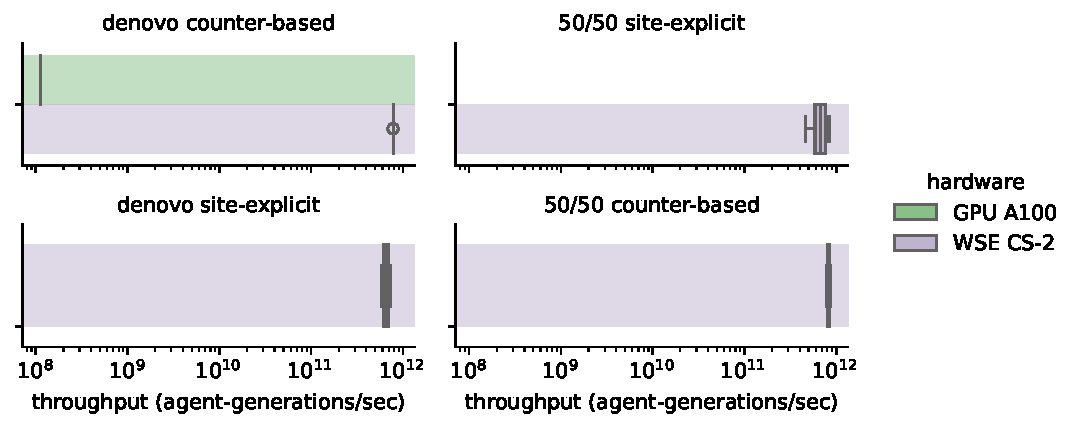
\includegraphics[width=\textwidth, trim={0cm 0cm 2.5cm 0cm}, clip]{binder/binder-perf-wse-vs-gpu.ipynb/binder/teeplots/col=experiment-design+hue=hardware+orient=h+viz=backplot+x=throughput-agent-generations-sec+ext=.pdf}
% \caption{throughput}
% \label{fig:perf:throughput}
% \end{subfigure}%
% \begin{subfigure}{0.49\textwidth}
\centering
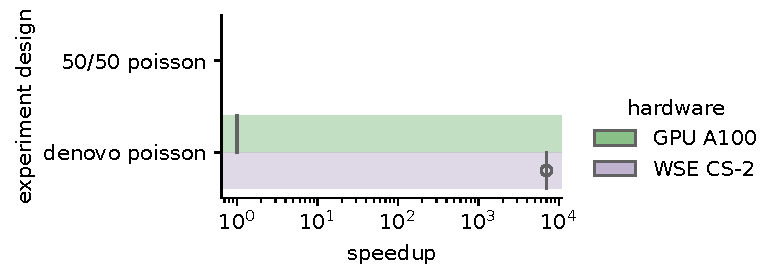
\includegraphics[width=0.85\linewidth]{binder/binder-perf-wse-vs-gpu.ipynb/binder/teeplots/hue=hardware+orient=h+viz=backplot+x=speedup+y=experiment-design+ext=.pdf}

\vspace{-2ex}
% ~
% \caption{speedup}
% \label{fig:perf:speedup}
% \end{subfigure}

\caption{
  \textbf{CPU, GPU, and WSE simulation performance.}
  \footnotesize
  CPU throughput was measured from NumPy-backed simulation code, GPU throughput was measured from equivalent CuPy-backed simulation code, and WSE throughput was measured from a comparable Cerebras Software Language implementation.
  CPU experiments were single-core on AMD EPYC 7H12 (2.595 GHz), GPU hardware was NVIDIA A100 hosted by AMD EPYC 7713 (2.0 GHz) or Intel Xeon 8358 (2.6 GHz), and WSE hardware was CS-2 hosted by Intel Xeon Platinum 8280L (2.7-4.0 GHz).
  Speedup was calculated relative to mean CPU throughput.
  % Shaded areas indicate bootstrapped 95\% confidence intervals with sample size $\geq 10$.
}
\label{fig:perf}
\end{figure}


To assess the efficacy of hardware accelerator resources in expediting our simulations, we collected timings of runtime duration from our simulation experiments.
As a baseline comparison point, we also benchmarked corresponding single-core CPU simulation code.

Mean throughput was 7.0 (std. deviation [SD] 0.5) million agent-generations per second (AGPS) on CPU, 2.7 (SD 0.03) billion AGPS on GPU, and 780 (SD 0.5) billion AGPS on WSE for \textit{de novo} trials using the counter-based model.
We found that WSE provided a speedup of $111,091\times$ (SD 75) over CPU and $294\times$ (SD 0.2) over GPU (Figure \ref{fig:perf}).
% Net speedup, normalized to mean CPU throughput, was $378\times$ (SD 4) on GPU and $111,091\times$ (SD 75) on WSE.
% Normalized to GPU performance, WSE provided a speedup of $294\times$ (SD 0.2).

% Under the site-explicit model, WSE gave 650 (SD 50) billion AGPS under \textit{de novo} conditions.
% The site-explicit model was not implemented on GPU.
% For all the above, 50/50 trials gave similar performance to \textit{de novo}.

On WSE, we found agent-generation throughput to be consistent across per-PE population densities.
%, as shown in Supplementary Figure \ref{fig:perf-tilepop}.
In contrast, on GPU we encountered an apparent memory-wall effect where mean throughput dropped $>95\%$ to 121 million AGPS when increasing net population size from 15.1 million to 175 million.
% For this reason, we only scaled GPU experiments up to 15.1-million-agent populations ($243 \times 243$ demes).

% \subsection{Major Results}

% In our initial experiment, we confirmed that large populations favor mutator fixation, under the assumption of unlimited adaptive potential.
% Consistent with expectations, we found that restricting adaptive potential by capping available adaptive mutations reversed outcomes in large populations to favor nonmutators.
% Investigating the influence of population structure and composition, we found spatial structure to substantially increase the amount of adaptive potential required to fix mutator alleles in large populations.
% However, this effect only occurred when mutator alleles were initially rare within the population.
% We also report qualitative differences between effects of population size on mutator fixation probability under well-mixed versus 2D population structure when mutations are rare.
% In the final part of our investigation, we analyze the spatiotemporal dynamics of our simulations to better understand the mechanisms at play behind these effects.

% Differing from existing results, we find that in the situation of limited adaptive potential, the effect of population structure on fixation probability is actually opposite to that predicted under the theory.
% Population structure has also been found to influence mutator outcomes, with deviation from well-mixed conditions being linked to a higher probability for hypermutator fixation so long as any connectivity remains between subpopulations \citep{raynes2019migration}.


% \section{Results and Discussion} \label{sec:results}

% In this work, we investigate the interactions between population size, adaptive potential, and population structure in influencing selection on mutator traits within asexual populations.
% In our first experiments, we replicate previous work by \citet{raynes2018sign} showing sign-change effects of population size on mutator favorability.
% Subsequent experiments investigate how these dynamics vary based on initial mutator abundance and the availability of beneficial mutations.
% Finally, experiments compare mutator dynamics between well-mixed population structure and spatial segregation into subpopulations connected by migration.

% \subsection{Scaling Population Size}
% \label{sec:scaling-population-size}

% In a first set of experiments, we tested the capability of our model to reproduce the qualitative regimes of mutator dynamics across population scales identified by \citet{raynes2018sign}.
% In the first regime, where population size is very small, fixation of mutator and nonmutator alleles is nearly equiprobable, owing to the overwhelming influence of stochastic effects.
% Subsequently, in medium-sized populations, mutators become disfavored on account of increased power of selection becoming in penalizing the increased mutational load imposed by mutator alleles.
% Finally, in sufficiently large populations, a sign-change fitness effect occurs and mutator fixation becomes overwhelmingly favored.
% This effect occurs in asexual populations because population size increases the probability of at least one mutator discovering a beneficial mutation, and so ``hitch-hiking'' to sweep out nonmutators.

% \begin{figure}[h]
  % adapted from https://tex.stackexchange.com/a/122813/316176
  \captionsetup[subfigure]{justification=raggedright}
  \begin{minipage}{0.7\textwidth}

    \begin{minipage}{0.04\textwidth}~\end{minipage}%
    \begin{minipage}{0.44\textwidth}
      \centering
      \itshape
      \textbf{unlimited} beneficial mutations
    \end{minipage}%
    \begin{minipage}{0.34\textwidth}
      \centering
      \itshape
      \textbf{single} beneficial mutation
    \end{minipage}

    ~\vspace{-1.5ex}

    % Top subfigure
    \begin{subfigure}[b]{\linewidth}
      \begin{minipage}{0.88\textwidth}
        \begin{minipage}{0.53\textwidth}
          \includegraphics[height=2.9cm, trim={0cm 0.2cm 3.5cm 0.8cm}, clip]{binder/binder-wse-5050-spatial2d-32atile-infben-traits.ipynb/binder/teeplots/wse-5050-spatial2d-32atile-infben-traits/errorbar=ci+hue=genotype+num-abm=(inf,)+style=genotype+viz=size-fixation-areaplot+x=population-size+y=fixation-probability+ext=.pdf}%
        \end{minipage}%
        \begin{minipage}{0.47\textwidth}
          \includegraphics[height=2.9cm, trim={1.3cm 0.2cm 3.5cm 0.8cm}, clip]{binder/binder-wse-5050-spatial2d-32atile-infben-traits.ipynb/binder/teeplots/wse-5050-spatial2d-32atile-infben-traits/errorbar=ci+hue=genotype+num-abm=(1.0,)+style=genotype+viz=size-fixation-areaplot+x=population-size+y=fixation-probability+ext=.pdf}
        \end{minipage}
      \end{minipage}%
      \hspace{-3ex}%
      \begin{minipage}{0.12\textwidth}
        \raggedright
        \caption{\footnotesize 32 agents per PE\\~\\~\\}
        \label{fig:wse-inf-one:32}
      \end{minipage}%
    \end{subfigure}%

    % Bottom subfigure - Adjusted layout to match the top
    \begin{subfigure}[b]{\linewidth}
      \begin{minipage}{0.88\textwidth}
        \begin{minipage}{0.53\textwidth}
          \includegraphics[height=2.9cm, trim={0cm 0.2cm 3.7cm 0.8cm}, clip]{binder/binder-wse-5050-spatial2d-2048atile-infben-traits.ipynb/binder/teeplots/wse-5050-spatial2d-2048atile-infben-traits/errorbar=ci+hue=genotype+num-abm=(inf,)+style=genotype+viz=size-fixation-areaplot+x=population-size+y=fixation-probability+ext=.pdf}%
        \end{minipage}%
        \begin{minipage}{0.47\textwidth}
          \includegraphics[height=2.9cm, trim={1.3cm 0.2cm 3.7cm 0.8cm}, clip]{binder/binder-wse-5050-spatial2d-2048atile-infben-traits.ipynb/binder/teeplots/wse-5050-spatial2d-2048atile-infben-traits/errorbar=ci+hue=genotype+num-abm=(1.0,)+style=genotype+viz=size-fixation-areaplot+x=population-size+y=fixation-probability+ext=.pdf}
        \end{minipage}
      \end{minipage}%
      \hspace{-3ex}%
      \begin{minipage}{0.1\textwidth}
        \caption{\footnotesize 2,048 agents per PE\\~\\~\\}
        \label{fig:wse-inf-one:2048}
      \end{minipage}%
    \end{subfigure}%

~\vspace{-1.2ex}

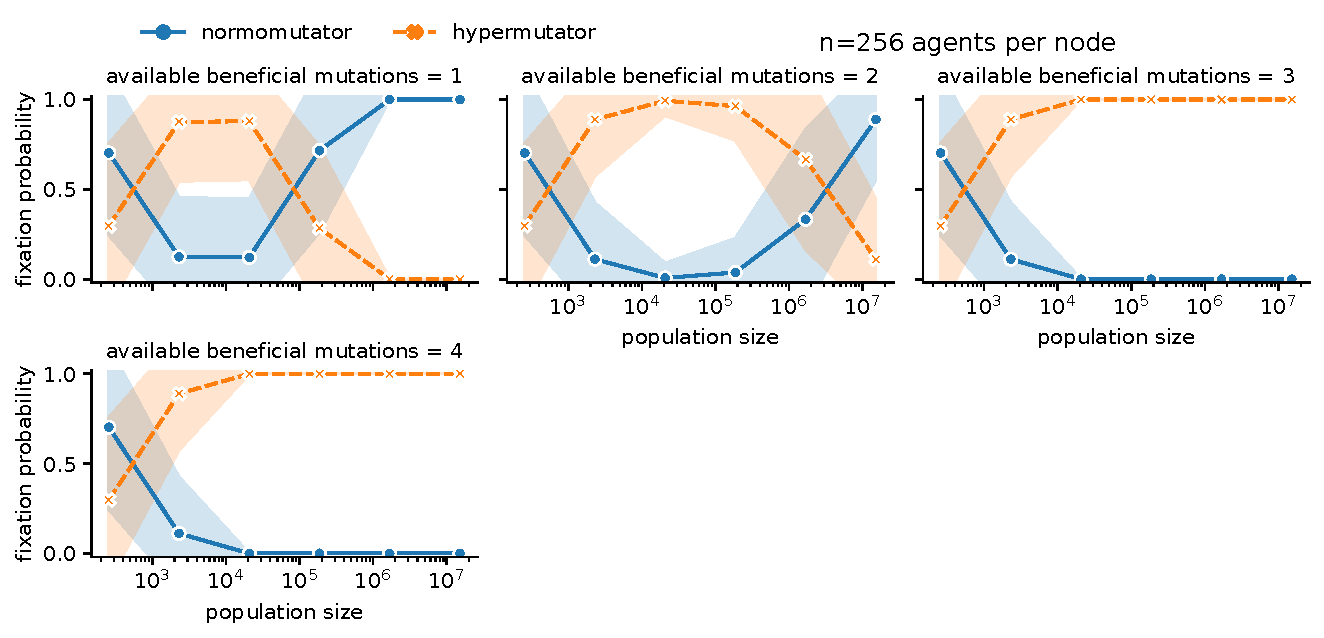
\includegraphics[width=0.9\textwidth, trim={0cm 4.7cm 6.2cm 0cm}, clip]{binder/binder-wse-5050-spatial2d-2048atile-infben-traits.ipynb/binder/teeplots/wse-5050-spatial2d-2048atile-infben-traits/col=available-beneficial-mutations+errorbar=sd+hue=genotype+kind=line+style=genotype+viz=relplot+x=population-size+y=fixation-probability+ext=}

  \end{minipage}%
  \begin{minipage}{0.3\textwidth}
    \caption{%
      \textbf{Restricted adaptive potential favors nonmutators in large populations.}
      \footnotesize
      Area plots compare mutator versus nonmutator fixation probabilities across surveyed population sizes.
      When adaptive potential is unlimited (left column), mutators are strongly favored in large populations, owing to their capacity to more rapidly discover beneficial mutations.
      Right column shows fixation outcomes across population sizes, with adaptive potential restricted to just one beneficial mutation.
      As before, mutators gain favor in intermediate population sizes.
      However, under the adaptation-restricted regime, nonmutators regain favor at very large population sizes.
      Top panel, \ref{fig:wse-inf-one:32}, shows results with subpopulation size of 32 agents per PE, scaling population size up to 23.9 million.
      Bottom panel, \ref{fig:wse-inf-one:2048}, reports 2,048 agents per PE with population sizes up to 1.5 billion.
      Experiments were conducted on WSE with counter-based genome model, using populations initialized with a 50/50 mix of non- and mutators.
      Error bands indicate bootstrapped 95\% confidence intervals.
      Supplementary Figure \ref{fig:fixheat-wse-altatile} details results in a tabular format.
    }
    \label{fig:wse-inf-one}
  \end{minipage}
\end{figure}


% As shown in the left panel of Figure \ref{fig:wse-inf-one:32}, our simulations reproduce the sign-change fitness effect described by \citet{raynes2018sign}.
% Leveraging the capabilities of WSE accelerator hardware, we tested population sizes several orders of magnitude beyond those reported in \citet{raynes2018sign}.
% For these experiments, 2D population structure was used with 50/50 initialization.
% In line with expectations, no further qualitative differences in mutator fixation probability emerged in these larger population sizes, which ranged up to 1 billion agents.
% For the largest-scale trials, shown in the left panel of Figure \ref{fig:wse-inf-one:2048}, an increased subpopulation size of 2,048 agents per deme was used.
% As such, in these trials, note that coarsened spacing between surveyed population sizes obscures the sign-change fitness effect near the lower bound of population size.

% \subsection{Restricting Adaptive Potential}
% \label{sec:restricting-adaptive-potential}

% \subsection{Major Results}

% \begin{figure*}

\begin{minipage}{0.65\textwidth}
  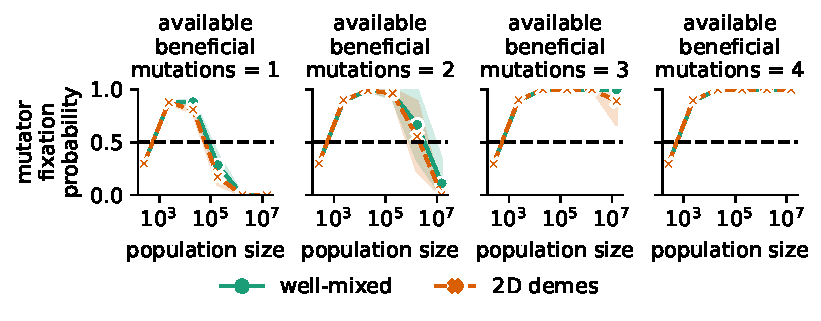
\includegraphics[width=\textwidth]{binder/binder-cupy-5050-traits.ipynb/binder/teeplots/cupy-5050-traits/col=available-beneficial-mutations+errorbar=ci+hue=population-structure+kind=line+palette=dark2+style=population-structure+viz=relplot+x=population-size+y=fixation-probability+ext=.pdf}%
\end{minipage}
\begin{minipage}{0.3\textwidth}
\caption{
\textbf{Well-mixed and spatially-structured populations exhibit similar relationship between population size and mutator fixation probability.}
\footnotesize
In both scenarios, as available beneficial mutations are increased, mutators gain favor in progressively larger population sizes.
Simulations were conducted on GPU using the counter-based genome model, with populations initialized to a 50/50 mix of non- and mutators.
Subpopulations comprised 256 agents per PE.
Shaded bands show bootstrapped 95\% confidence intervals.
}
\label{fig:avail-ben-muts-gen}
\end{minipage}

\end{figure*}


% Given that experiments conducted on the WSE platform all involve 2D spatial structure, we implemented an additional set of GPU-based experiments to compare findings with well-mixed population structure.
% Figure \ref{fig:avail-ben-muts-gen} overviews these results.
% Although experiments ranged up to a smaller maximum population size on the GPU platform, detected regimes of mutator dynamics are consistent with WSE-based experiments.
% Comparing on the basis of spatial structure, we find fixation probabilities to be near-identical between GPU-based trials using 2D and well-mixed structure across surveyed conditions.
% % https://github.com/mmore500/hypermutator-dynamics/blob/484ac79f35baf10e4acc52babee836d10ab50bdb/binder/cupy-5050-traits.ipynb
% We find significant divergence in fixation probability between spatial structure treatments only for population size 20,736 with adaptive potential of one available beneficial mutation (Mann-Whitney U test; $p < 0.0005$; Bonferroni corrected $p < 0.01$).

% \subsection{Effects of Background Mutator Prevalence}
% \label{sec:background-hypermutator-prevalence}

% \input{fig/denovo-5050-conditions-combined}

% Having observed large population size prevent mutator fixation in competition experiments under conditions of limited adaptive potential, we next sought to assess how such an effect might manifest in more naturalistic conditions.
% For this purpose, we relaxed the initial condition that mutators begin ``50/50'' in equal proportion to nonmutators.
% Instead, we allowed mutators to enter the population at a low background rate \citep{desai2011balance,johnson1999approach}, an experimental design common with several previous simulation studies of hypermutator dynamics \citep{wylie2009fixation,tenaillon1999mutators}.
% To provide a conservative reflection of the impact of mutator allele rarity, we used a mutator allele introduction probability of $10^{-6}$ per replication event.
% Figure \ref{fig:denovo-5050-conditions-combined} compares mutator fixation probabilities between 50/50 and \textit{de novo} conditions.
% Trials were conducted with 2D spatial structure on the WSE platform.
% With 256 agents per deme, population size scaled up to 136 million agents.

% Prior work analyzing conditions with infinite adaptive potential has shown per-capita favorability of mutator traits to be density independent \citep{raynes2019selection}.
% As such, a lower background rate for mutator alleles should be expected to substantially reduce the net probability of mutator fixation.
% In line with expectations, the \textit{de novo} treatment substantially reduces mutator fixation.
% Under \textit{de novo} conditions, nonmutators reliably resist mutator fixation in populations of 136 million through more than 10 beneficial mutations available.
% Under 50/50 conditions, by contrast, mutators begin to fix in these large populations past 2 beneficial mutations available.

% We performed sensitivity analysis of our findings to the underlying counter-based genome model used.
% For this purpose, we implemented an alternate ``site-explicit'' model where the probability of discovering a beneficial mutation scales proportionally to the number available.
% As shown in Supplementary Figure \ref{fig:wse-site-explicit-counter-based}, results were generally consistent between the two genome models.
% Notably, though, under the ``site-explicit'' model, mutator alleles are more frequently fixed within the smallest surveyed population size under 50/50 initialization.

% % ^^^ https://github.com/mmore500/hypermutator-dynamics/blob/5e904ac2fbbd4b41a0ad679883fc1a63af71c00c/binder/wse-denovo-spatial2d-explicitsite-timeseries.ipynb
% To assess the magnitude of transient peak mutator concentrations across levels of adaptive potential, we performed an additional set of four-replicate simulations with adaptive potentials ranging from 2 to 10 available beneficial mutations.
% For all replicates with 6 or more available beneficial mutations, mutators peaked beyond 50\% prevalence (Figure \ref{fig:peaksweep}).

% \subsection{Effects of Population Structure}
% \label{sec:population-structure}

% In a final set of experiments, we extended our earlier trials with 50/50 initialization to assess the impact of spatial structure on mutator dynamics where mutators are initially rare.
% In particular, we were curious whether removal of population structure would negligibly affect mutator fixation probabilities, as was earlier the case with 50/50 initialization.
% Trials conducted in this experiment comparing the 2D deme structure to fully well-mixed conditions were conducted using GPU evaluation.
% As a result, population sizes ranged only up to 15 million.

% \input{fig/spatial-structure-combined}

% Figure \ref{fig:spatial-structure-combined} plots increase in mutator fixation probability with available adaptive potential across a spectrum of population sizes.
% Interestingly, spatial structure does cause results to differ substantially under \textit{de novo} conditions.
% We find that in large nonmutator populations of 15 million with well-mixed structure, fixation probability of mutator alleles becomes appreciable with adaptive potential of only 5 available beneficial mutations.
% This is not the case for large populations with 2D deme structure, where fixation of mutator alleles become appreciable above 10 available beneficial mutations.
% For intermediate population sizes of 186,000 agents, however, an opposite effect occurs: spatial structure raises the probability of mutator fixation across the board of available adaptive potential compared to well-mixed conditions.

% These findings contrast with previous modeling work assuming unlimited adaptive potential, which predicts that so long as any level of connectivity exists between subpopulations, spatial structure boosts mutator fixation probability \citep{raynes2019migration}.
% One possible explanation for why spatial structure can decrease mutator fixation probability is in extending fixation times, which extends the opportunity for nonmutators to exploit available adaptive potential before being driven to extinction.
% This described effect notably aligns with findings from \textit{in vivo} evolution experiments with \textit{E. coli} that show that migration barriers delaying introduction of mutator strains into nonmutator populations can reduce mutator advantage \citep{lechat2006escherichia}.

% On a separate front, it is surprising that substantial differences in mutator dynamics between deme-structured and well-mixed conditions only become apparent with low initial mutator frequency, given the established expectation of fitness effects of mutator alleles as a density- and number-independent \citep{raynes2019selection}.
% While one possible explanation may be in part that detectability of fitness effect magnitudes is masked by sensitivity limitations of the 50/50 assay, this result draws into question the extent to which density-independence of mutator fitness effects generalizes to scenarios with limited adaptive potential and spatial structure.
% In future work, it would be informative to test whether the impact of spatial structure where mutators are rare stems from heterogeneity in the spatial distribution of mutator clades or from slowing the spread of beneficial alleles.


\section{Conclusion} \label{sec:conclusion}


% Mutations are fundamental drivers of evolution, generating the genetic diversity necessary for populations to adapt and survive \citep{hershberg2015mutation}.
% Developing this understanding is important Understanding the factors that influence selection on mutation rates themselves is therefore key in understanding and managing evolutionary dynamics within asexual populations.
% Ongoing efforts have established an increasingly detailed theoretical basis to explain how selection and drift effects act on alleles modifying mutation rate.
% In particular, existing theory provides a rigorous understanding of how alleles that increase mutation rate can become abundant in asexual populations by way of hitchhiking on discovered of beneficial mutations, particularly when population size is large.
% However, less detailed understanding exists as to factors that suppress mutator alleles within large asexual populations.
% In this work, we have applied simulation experiments to investigate how adaptive potential and population structure influence mutator dynamics, including mediation of sign change fitness effects in large populations.

% This work contributes experiments to better characterize factors affecting selection on mutator traits in very large populations.
% replicated the sign-change effect of population size on mutator fixation probability, and
% In a first set of experiments, we confirmed that, under the assumption of unlimited adaptive potential, increases in population size transition outcomes to a regime where mutators become strongly favored.
% However, we found that restricting adaptive potential reversed outcomes in very large populations, creating a tertiary regime where nonmutators regain selective favor.
% This effect appeared consistently under both a simple counter-based genome model, adapted from \citet{raynes2018sign}, and a more detailed ``site-explicit'' genome model where alleles with potential to experience adaptive mutation were tracked directly.

% Subsequent experiments investigated the influence of population structure and composition on adaptation-constrained mutator dynamics.
% We found outcomes to be highly sensitive to baseline frequency of mutators.
% When mutators were initially rare, mutator fixation was suppressed in large populations through substantially more available adaptive mutations.
% Spatial structure further amplified these effects, but only when mutators were initially rare.

% Much future work remains.
% One phenomenon in some benchtop evolution experiments \citep{ho2021evolutionary}, but not considered in present work, is mutator reversion.
% In a reversion scenario, gain-of-function mutations restore a mutator strain toward baseline nonmutator rates, either partially or fully.
% Crucially, reversion events introduce the possibility of escape from otherwise permanent mutator fixation \citep{taddei1997role}.
% Even when rare, reversion can significantly influence mutator dynamics.
% For instance, low-frequency recombination processes that facilitate restoration of DNA repair mechanisms can strongly influence the fate of mutators \citep{tenaillon2000mutators}.

% Given experimental evidence highlighting limitations of mutator strategies in facilitating adaptation within complex environments \citep{ho2021evolutionary}, another informative extension would be to explore how mutator dynamics manifest within richer fitness landscapes that capture aspects of pleiotropy, redundancy, and asymmetry.
% Within this framework, it would be possible to study adaptive potential in terms of distortions of fitness landscape topology, rather than artificial caps on available beneficial mutations.
% Models of adaptive potential with an asymptotic, rather than capped, supply of beneficial mutations might also be explored.

Use of hardware accelerator technology for high-performance computing was key in enabling agent-based simulation at the population scales explored in this work.
However, further work remains in algorithm and software development to leverage these platforms for \textit{in silico} evolution experiments.
For example, although trivial for GPU architecture, implementing well-mixed (or nearly well-mixed) migration on WSE hardware will necessitate densely connected, hierarchical, or fully point-to-point routing structures among processor elements \citep{james2020physical,luczynski2024near}.
Across all future experiments, insight could be deepened by tracking phylodynamics within simulated populations.
Recent work has demonstrated potential for lightweight reconstruction-based strategies for phylogenetic tracking in many-processor evolution simulations \citep{moreno2024trackable}.
%, important methods development work remains in providing sufficient tree reconstruction throughput to enable large-scale analyses \citep{moreno2024trackable}.
% Such an approach might ultimately incorporate implementation for runtime sampling of genomes from device to host, to serve as ``fossils'' in revealing intermediate phenotypic characters and fleshing out the lineage structure of extinct clades \citep{moreno2024guide}.
% Findings from this work highlight the role of available adaptive potential, in conjunction with spatial structure and background mutator frequency, in influencing the evolution of mutation rates in asexual populations.
% In concert with empirical data from \textit{in vivo} experiments, simulation studies are key in guiding development of formal descriptions explaining relationships among evolutionary dynamics --- as has been accomplished in earlier model-based investigations of mutator dynamics \citep{wylie2009fixation,raynes2018sign}.
% In the case of present work, such formulations seem likely to largely revolve around projections of mutation waiting times and time to fixation for beneficial alleles \citep{ribeck2016competition}.
% Further, in the face of scenarios involving extensive mechanistic complications, agent-based simulations can supplement mathematical approaches as predictive instruments in their own right \citep{an2009agent}.
To this end, we see work increasing the feasible scale of simulation by leveraging accelerator hardware as a key contributing step in broader development of more powerful predictive capabilities for the behavior of real-world biological systems.
% Ultimately, very large-scale simulations may drive so-called ``digital twins'' of evolving populations --- high-fidelity computational models that incorporate real-time feedback to mirror their physical counterpart \citep{dekoning2023digital}.
% Such digital twins will not only advance our theoretical insights but also provide practical tools for predicting and controlling evolutionary trajectories in natural and artificial populations.
% We expect that developments in this vein will play a role in addressing complex biological challenges in medicine, public health, and natural resources management, as well as enriching our understanding of evolution in an ever-changing world.



% \input{text/acknowledgement.tex}

\renewcommand\bibfont{\scriptsize}
\putbib


\end{bibunit}

% \clearpage
% \newpage

% \begin{bibunit}

% \input{text/supplement.tex}

% \renewcommand\bibfont{\scriptsize}
\putbib


% \end{bibunit}

\end{document}
